\documentclass[a4paper,12pt]{article}
\usepackage[utf8]{inputenc}
\usepackage[T1]{fontenc}
\usepackage{geometry}
\geometry{margin=1in}
\emergencystretch=3em
\usepackage[table]{xcolor}
\usepackage{graphicx}
\usepackage{fancyhdr}
\usepackage{lmodern}
\usepackage{tocloft}
\usepackage{enumitem}
\usepackage{titlesec}
\usepackage{caption}
\usepackage{subcaption}
\usepackage{amsmath}
\usepackage{float}
\usepackage[english]{babel}
\usepackage{hyperref}
\usepackage[outputdir=.]{minted}
\usepackage{minted}

% --- Report accent colours ---
\definecolor{figblue}{RGB}{15,76,129}     % dark blue for figure labels
\definecolor{tabgreen}{RGB}{30,102,56}    % dark green for table labels
\definecolor{linknavy}{RGB}{30,58,138}    % navy for hyperlinks
\definecolor{citemaroon}{RGB}{128,28,28}  % maroon for citations

% --- Caption styling: coloured labels, small italic body ---
\captionsetup{labelsep=colon, font=small, textfont=it}
\captionsetup[figure]{labelfont={bf,color=figblue}}
\captionsetup[table]{labelfont={bf,color=tabgreen}}
\captionsetup[sub]{font=footnotesize, labelfont={bf,color=figblue}, textfont=it}

% --- Section heading colours (navy for sections, softer navy for subsections) ---
\titleformat{\section}{\normalfont\Large\bfseries\color{linknavy}}{\thesection}{1em}{}
\titleformat{\subsection}{\normalfont\large\bfseries\color{linknavy!80!black}}{\thesubsection}{1em}{}

% --- Coloured callout for in-paragraph summary headers ---
\newcommand{\callout}[1]{\textbf{\textcolor{tabgreen}{#1}}}

% --- Hyperref styling: coloured links instead of garish boxes ---
\hypersetup{
    colorlinks=true,
    linkcolor=linknavy,
    citecolor=citemaroon,
    urlcolor=linknavy,
    filecolor=linknavy
}

\usepackage[normalem]{ulem}
\newcommand{\redsout}[1]{\textcolor{red}{\sout{\textcolor{black}{#1}}}}

\definecolor{mintedbg}{RGB}{245,245,240}
\definecolor{mintedframe}{RGB}{210,210,210}
\usemintedstyle{friendly}
\setminted{
    bgcolor=mintedbg,
    frame=single,
    framesep=2mm,
    rulecolor=\color{mintedframe},
    breaklines=true,
    fontsize=\small
}

\pagestyle{fancy}
\fancyfoot[C]{\thepage}
\fancyhead[L]{\textit{Facultat d'Informàtica de Barcelona — Master's in Artificial Intelligence}\\ \textbf{Advanced Human Language Technologies (AHLT)}}
\fancyhead[R]{2025--2026}
\makeatletter
\let\ps@plain\ps@fancy
\makeatother

\begin{document}
\begin{titlepage}
    \thispagestyle{fancy}
    \centering
    \vspace*{-0.8cm}

    \begin{center}
\begin{minipage}[c]{0.35\linewidth}
    \centering
    
\includegraphics[height=1.8cm,keepaspectratio]{UPC-2.png}
\end{minipage}%
\begin{minipage}[c]{0.35\linewidth}
    \centering
    
\includegraphics[height=1.8cm,keepaspectratio]{fib.png}
\end{minipage}
\end{center}


  \vspace{0.2cm}
{\LARGE\bfseries AHLT Lab Project Report \\[0.15cm]
\textit{Task 1 — NERC (Named Entity Recognition and Classification)}}\\[0.3cm]

\begin{center}
\begin{tabular}{@{}l @{\hspace{2cm}} l @{\hspace{2cm}} l@{}}
\textbf{Authored by:} & \textbf{Lab Group:} & \textbf{Date:} \\
Ralph Khairallah (Exchange)      & 10                     & \today \\
Francesco Dorati (Exchange)      &                        &        \\
\end{tabular}
\end{center}

\vspace{0.3cm}

\begin{center}
    \textcolor{linknavy}{\textbf{\huge\scshape Contents}}
\end{center}

\vspace{-0.6cm}

    \renewcommand{\contentsname}{}
    \renewcommand{\cftsecfont}{\bfseries\Large}
    \renewcommand{\cftsubsecfont}{\normalfont\large}
    \setlength{\cftbeforesecskip}{10pt}
    \setlength{\cftbeforesubsecskip}{5pt}
    \setcounter{tocdepth}{2}
    \tableofcontents

\end{titlepage}

\setcounter{page}{3}

% =============================
% AHLT Lab Project (Task 1: NERC)
% Structure + table of contents aligned with AHLTLabProject.pdf.
% Only System 1.1 is completed at this stage.
% =============================

\section{Introduction}

\subsection{Context}
Drug--drug interactions (DDIs) are a leading cause of adverse
clinical events, and most of the evidence for them lives in
unstructured biomedical text: drug labels, case reports, scientific
abstracts. Before any interaction can be extracted, the drugs
themselves must be located and classified --- a Named Entity
Recognition and Classification (NERC) problem. The task is harder
than generic NER because drug names are highly productive (new
compounds appear constantly), they share surface features with
ordinary English words (\textit{aspirin}, \textit{caffeine}), and
four distinct sub-types (approved drugs, brand names, drug groups,
unapproved / experimental compounds) must be told apart. This
report addresses the NERC sub-task of SemEval-2013 Task~9
(DDIExtraction), using the DrugBank $+$ MedLine corpus provided by
the shared task.

\subsection{Objectives}
The project delivers and compares three NERC systems spanning the
main paradigms in modern NLP:
\begin{itemize}[nosep]
    \item \textbf{System 1.1 --- feature-based Machine Learning}:
          CRF, SVM and MaxEnt classifiers on hand-crafted features
          (morphology, PoS, dictionary lookups).
    \item \textbf{System 1.2 --- Neural Networks}: a BiLSTM tagger
          with configurable input representations (word /
          lower-cased word / suffix / prefix / lemma / PoS /
          binary features) and architecture knobs.
    \item \textbf{System 1.3 --- Large Language Models}: a
          generative XML-tagging approach, evaluated both few-shot
          (no training) and after LoRA fine-tuning on quantised
          Llama-3.2-3B and Qwen-2.5-3B.
\end{itemize}
For each system we document the input representation, architecture
and hyperparameter exploration, the development-set selection
protocol, and the final test-set numbers. A closing cross-system
comparison (§\ref{sec:conclusions}) discusses the four dimensions
required by the lab specification: \emph{effort},
\emph{computational cost}, \emph{explainability /
controllability}, and \emph{performance}.

\section{Data, evaluation, and reproducibility}

\subsection{Dataset}
The dataset comes from the DDI Extraction 2013 shared task (SemEval-2013 Task~9). It consists of biomedical texts annotated with drug entity mentions. Each entity is classified into one of four types:

\begin{itemize}[nosep]
    \item \textbf{drug}: approved generic drug names (e.g., \textit{aspirin}, \textit{ibuprofen}).
    \item \textbf{brand}: commercial/trade names (e.g., \textit{Advil}, \textit{Tylenol}).
    \item \textbf{group}: pharmacological drug classes (e.g., \textit{NSAIDs}, \textit{opioids}).
    \item \textbf{drug\_n}: unapproved or experimental substances.
\end{itemize}

The data is split into three XML files:

\begin{table}[H]
\centering
\begin{tabular}{l r r}
\hline
\textbf{Split} & \textbf{Sentences} & \textbf{Entities} \\
\hline
Train  & 5{,}343 & 11{,}452 \\
Devel  & 1{,}477 & 3{,}125 \\
Test   & 1{,}455 & 3{,}228 \\
\hline
\end{tabular}
\caption{Dataset statistics.}
\label{tab:dataset}
\end{table}

\subsection{Evaluation protocol}
The task is formulated as \textbf{BIO sequence labeling}: each token is tagged as \texttt{B-}\textit{type} (beginning of an entity), \texttt{I-}\textit{type} (inside), or \texttt{O} (outside). The provided evaluator reconstructs entity spans from these tags and computes precision, recall, and F1 at the entity level. An entity is correct only if \emph{both} its span boundaries and its type match the gold standard (strict evaluation).

The evaluator reports two averages: \textbf{macro-averaged F1} (M.avg), which averages F1 across the four entity types equally, and \textbf{micro-averaged F1} (m.avg), which pools all predictions. Since the type distribution is heavily skewed (\textit{drug} accounts for $\sim$67\% of entities), macro-average is more sensitive to rare types like \textit{drug\_n}. Throughout this report, ``F1'' refers to \textbf{macro-averaged F1} (M.avg), as this is the primary metric reported by the evaluator.

\subsection{Reproducibility}
All code is in \texttt{code/1.1.NERC-ML/}. The pipeline is driven by \texttt{bin/run.py}, which supports three steps: \texttt{extract} (feature extraction), \texttt{train}, and \texttt{predict}. Feature toggles are controlled by boolean flags at the top of \texttt{bin/extract\_features.py}.

Hyperparameter sweep results are stored in \texttt{hyperparameter\_results\_mod*.csv}. Test evaluation scripts are \texttt{run\_best\_on\_test.sh} and \texttt{run\_mod8\_fast.sh}.

% ============================================================
\section{System 1.1 — NERC with Machine Learning}
% ============================================================

\subsection{Baseline}
The baseline system uses minimal token-level features: the word form, its lowercase version, suffixes (3 and 4 characters), and simple boolean flags (uppercase, title case, digit, contains dash/digit). Context features are limited to the immediate previous and next tokens. The baseline also checks single-token dictionary membership against an external drug lexicon.

Three classifiers are compared throughout:
\begin{itemize}[nosep]
    \item \textbf{CRF}: Conditional Random Fields (\texttt{pycrfsuite}), which model label sequences.
    \item \textbf{SVM}: Support Vector Machine (\texttt{sklearn.svm.SVC}), token-level classification.
    \item \textbf{MEM}: Maximum Entropy / Logistic Regression
    via \texttt{sklearn.linear\_model}.
\end{itemize}

Baseline devel results (default hyperparameters): CRF 67.9\%, SVM 67.1\%, MEM 65.5\%.

\subsection{Feature engineering experiments}

We incrementally added nine groups of features. Each modification was evaluated on the devel set with default hyperparameters. Table~\ref{tab:feature-mods} summarizes the modifications and Figure~\ref{fig:feature-evolution} shows the progression.

\begin{table}[H]
\centering
\small
\begin{tabular}{c l p{7.5cm}}
\hline
\textbf{Mod} & \textbf{Category} & \textbf{Features added} \\
\hline
1 & Token shape & Prefixes (2--4 chars), suffix-2, word shape, length buckets, punctuation flags (parens, slash, dot, plus, comma), dictionary membership flag \\
2 & POS tags & Part-of-speech (\texttt{tag\_}) and universal POS (\texttt{pos\_}) via spaCy \\
3 & Lemma & Lemma feature via spaCy lemmatizer \\
4 & Context POS & POS/lemma for $\pm$1 context tokens \\
5 & Window $\pm$2 & Full feature set for tokens at positions $i\pm2$ \\
6 & Biomedical patterns & Digit normalization, Greek letter detection, Roman numeral flag, chemical-like pattern, stereochemistry marker, dose unit flag \\
7 & Char n-grams & Character 3/4/5-grams for current token (capped at 8) \\
8 & Multi-token spans & Dictionary lookup for 2--5 token phrases with Begin/Inside/End markers \\
9 & Longer affixes & Prefix and suffix of length 5 and 6 characters \\
\hline
\end{tabular}
\caption{Feature modifications applied incrementally. Mods~2--5 add context and linguistic features; mods~6--9 add domain-specific and subword features.}
\label{tab:feature-mods}
\end{table}

\begin{figure}[H]
    \centering
    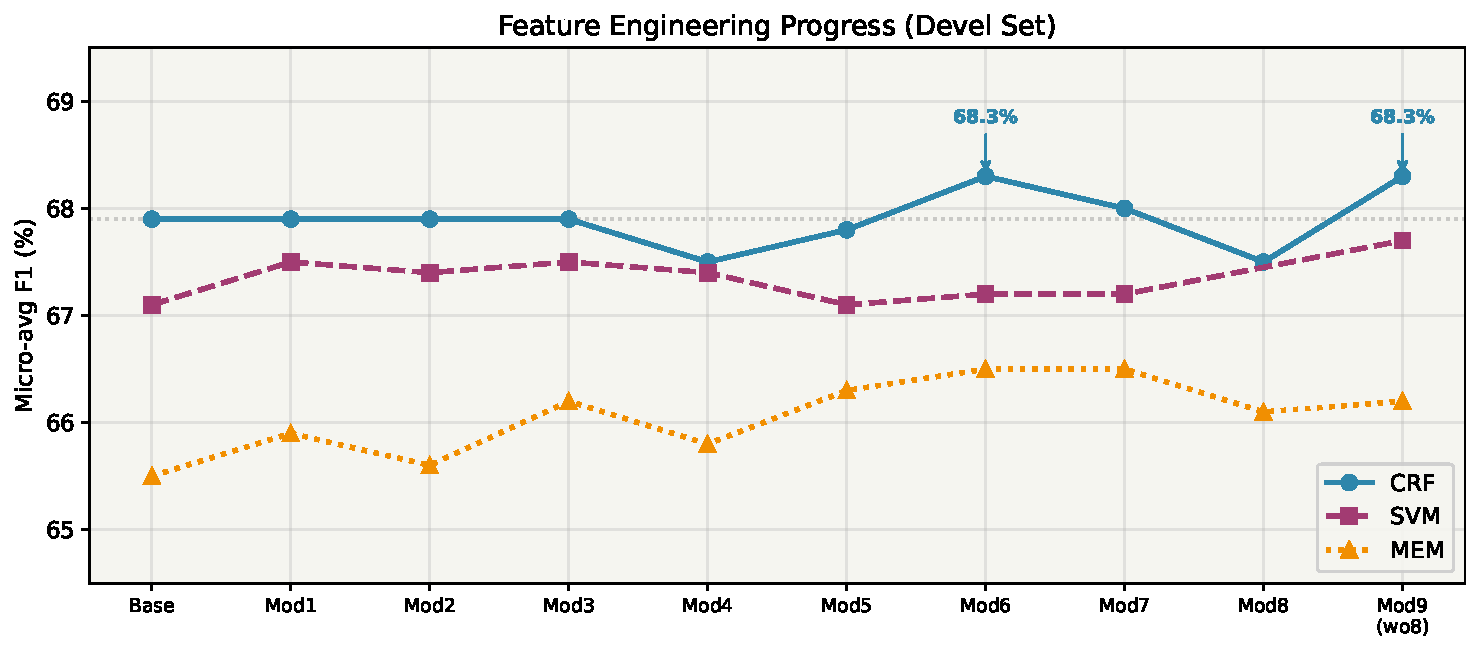
\includegraphics[width=\linewidth]{fig_feature_evolution.pdf}
    \caption{Devel set F1 across feature modifications for the three classifiers. CRF peaks at mod6 and mod9 (68.3\%). SVM improves steadily. MEM plateaus around 66\%.}
    \label{fig:feature-evolution}
\end{figure}

\callout{Key observations:}
\begin{itemize}[nosep]
    \item Mod~6 (biomedical patterns) gave the largest single improvement for CRF: +0.4 points.
    \item Mod~4 (context POS) unexpectedly \emph{hurt} CRF ($-$0.4 pts), likely due to feature space explosion with limited data. Reverting to mod~3 context and expanding the window ($\pm$2) in mod~5 was more effective.
    \item Mod~8 (multi-token spans) hurt CRF on devel but later proved beneficial on test (see Section~\ref{sec:test-eval}).
    \item MEM was insensitive to most feature additions, suggesting it struggles with the high-dimensional sparse feature space.
\end{itemize}

\subsection{Algorithm comparison (CRF, MEM, SVM)}

On the devel set, CRF consistently outperformed SVM and MEM across all feature configurations. However, this ranking did \emph{not} hold on the test set (Section~\ref{sec:test-eval}), highlighting the importance of final evaluation on held-out data.

\begin{table}[H]
\centering
\begin{tabular}{l c c c}
\hline
 & \textbf{CRF} & \textbf{SVM} & \textbf{MEM} \\
\hline
Best devel F1 (any mod) & \cellcolor{green!15}\textbf{68.5\%} & 67.7\% & 66.5\% \\
Best test F1 (mod8) & \cellcolor{green!15}\textbf{68.2\%} & 67.9\% & 67.8\% \\
\hline
\end{tabular}
\caption{Best F1 per algorithm on devel (after hyperparameter tuning) and test (mod8 features).}
\label{tab:algo-comparison}
\end{table}

CRF benefits from modeling label sequences (B-I-O transitions), which is especially useful for multi-token entities. SVM and MEM classify tokens independently but proved more robust to distribution shift between devel and test.

\subsection{Hyperparameter experiments}

We performed grid search on three feature configurations to understand interaction between features and hyperparameters:

\begin{itemize}[nosep]
    \item \textbf{mod6}: additions 1--6 (no char n-grams, no spans, no long affixes)
    \item \textbf{mod8}: additions 1--8 (includes char n-grams and multi-token spans)
    \item \textbf{mod9\_wo8}: additions 1--7 + 9 (char n-grams and long affixes, no spans)
\end{itemize}

\textbf{CRF} was tuned over $c_1 \in \{0.01, 0.1, 0.5, 1.0\}$, $c_2 \in \{0.1, 0.5, 1.0, 5.0\}$, and max iterations $\in \{50, 100, 200, 500\}$ (64 configurations per feature set).

\textbf{SVM} was tuned over $C \in \{0.1, 1.0, 10.0, 100.0\}$ and kernel $\in \{\text{linear}, \text{rbf}, \text{poly}\}$.

\textbf{MEM} was tuned over $C \in \{0.01, 0.1, 1.0, 10.0, 100.0\}$.

Figure~\ref{fig:crf-heatmap} shows the CRF hyperparameter landscape on mod6 (best devel feature set).

\begin{figure}[H]
    \centering
    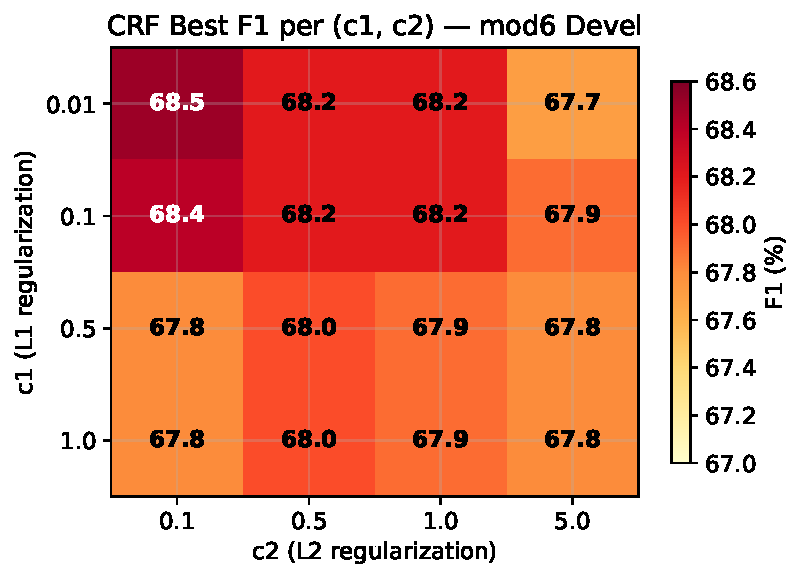
\includegraphics[width=0.55\linewidth]{fig_crf_heatmap.pdf}
    \caption{CRF devel F1 as a function of $c_1$ and $c_2$ (mod6, best iteration per cell). Low $c_1$ with low $c_2$ yields the best results. Performance is relatively stable across the grid ($\pm$1\%).}
    \label{fig:crf-heatmap}
\end{figure}

\callout{Key findings from hyperparameter tuning:}
\begin{itemize}[nosep]
    \item CRF: low regularization ($c_1 \leq 0.1$, $c_2 \leq 0.5$) with few iterations (50) works best. The model converges quickly.
    \item SVM: rbf kernel with $C = 0.75$--$1.0$ and default $\gamma$ (\texttt{scale}) is optimal. Manually setting $\gamma$ consistently hurts and can make training extremely slow (hours per run).
    \item MEM: completely insensitive to hyperparameters --- F1 stays at $\sim$66\% regardless of $C$ or iterations.
    \item The scores are tightly clustered within each model type ($<$1\% spread), meaning \textbf{the feature set matters more than hyperparameter tuning}.
\end{itemize}

\subsection{Best obtained results and discussion}
\label{sec:test-eval}

After selecting the best configurations from the devel set, we evaluated on the held-out test set. The results revealed a critical insight: \textbf{devel performance was a poor predictor of test performance} for CRF with mod6/mod9 features.

\begin{figure}[H]
    \centering
    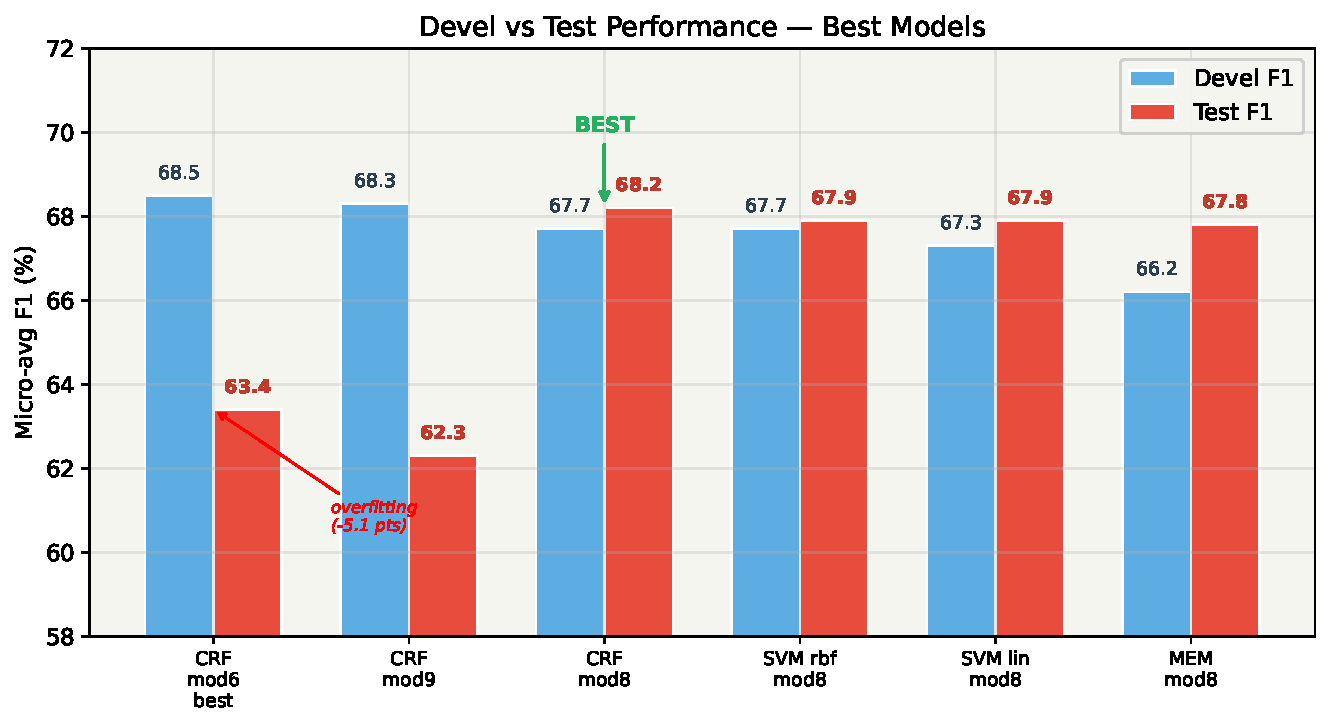
\includegraphics[width=\linewidth]{fig_devel_vs_test.pdf}
    \caption{Devel vs.\ test F1 for the best models. CRF on mod6/mod9 drops $\sim$5 points (overfitting). All mod8 models generalize well. The annotation ``BEST'' marks CRF mod8 at 68.2\% test F1.}
    \label{fig:devel-vs-test}
\end{figure}

Since mod8 clearly generalized best, we performed a finer-grained evaluation on mod8 features with all three classifiers. Figure~\ref{fig:svm-sensitivity} shows SVM robustness to $C$.

\begin{figure}[H]
    \centering
    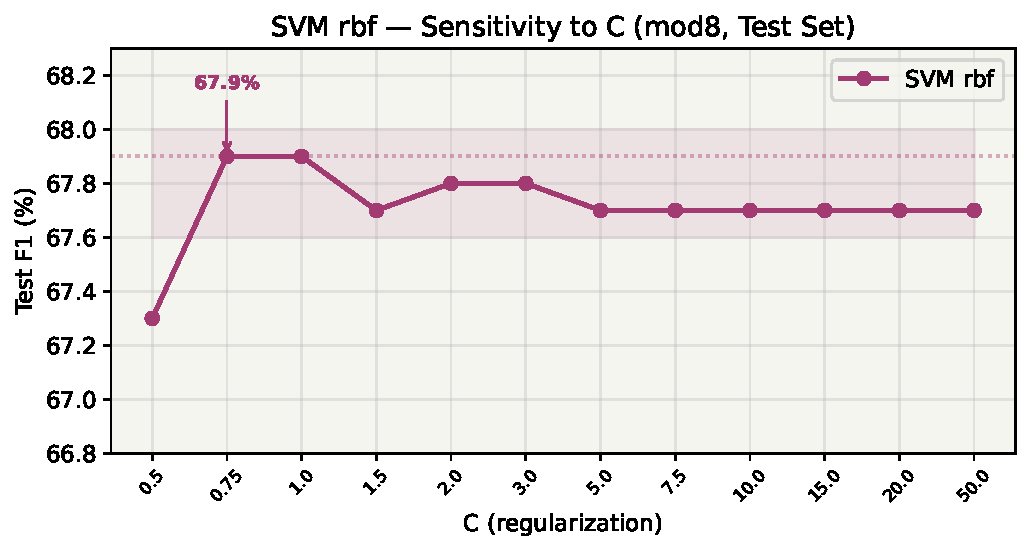
\includegraphics[width=0.75\linewidth]{fig_svm_c_sensitivity.pdf}
    \caption{SVM rbf test F1 across $C$ values (mod8 features). Performance is stable in the range $C \in [0.75, 50]$, peaking at $C = 0.75$--$1.0$ with 67.9\%.}
    \label{fig:svm-sensitivity}
\end{figure}

\begin{figure}[H]
    \centering
    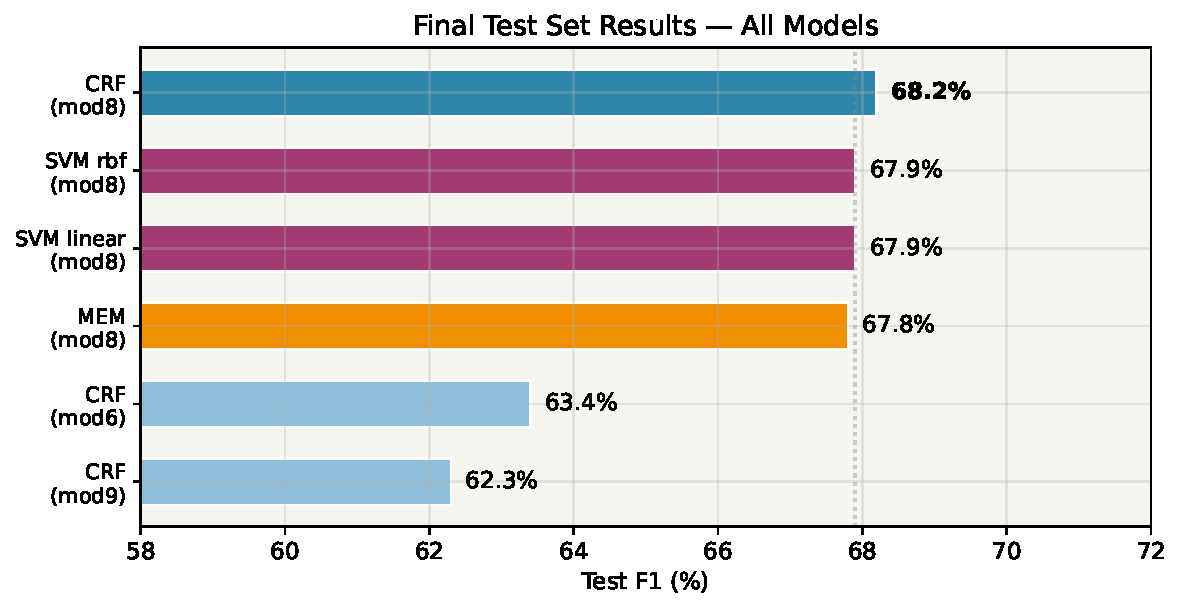
\includegraphics[width=0.85\linewidth]{fig_final_results.pdf}
    \caption{Final test set F1 for all evaluated models. Mod8 features yield the best generalization across all classifiers. CRF with mod6/mod9 features (light blue) overfit significantly.}
    \label{fig:final-results}
\end{figure}

Table~\ref{tab:final-results} summarizes the final test results.

\begin{table}[H]
\centering
\begin{tabular}{l l l c}
\hline
\textbf{Model} & \textbf{Features} & \textbf{Best hyperparameters} & \textbf{Test F1} \\
\hline
\rowcolor{green!18} CRF & mod8 & $c_1 = 0.1$, $c_2 = 0.1$, iter $= 50$ & \textbf{68.2\%} \\
SVM (rbf)    & mod8 & $C = 0.75$, $\gamma$ = scale & 67.9\% \\
SVM (linear) & mod8 & $C = 0.2$ & 67.9\% \\
MEM          & mod8 & $C = 1.0$ & 67.8\% \\
\hline
\rowcolor{red!10} CRF & mod6 & $c_1 = 0.01$, $c_2 = 0.1$, iter $= 50$ & 63.4\% \\
\rowcolor{red!10} CRF & mod9\_wo8 & $c_1 = 0.1$, $c_2 = 0.5$, iter $= 200$ & 62.3\% \\
\hline
\end{tabular}
\caption{Final test set results. The best model is \textbf{CRF with mod8 features at 68.2\% F1}. All mod8 models generalize well (67.8--68.2\%). CRF with mod6/mod9 features overfit.}
\label{tab:final-results}
\end{table}

\callout{Discussion:}
\begin{itemize}[nosep]
    \item \textbf{CRF mod8 is the best model} (68.2\% test F1), but the gap to SVM and MEM on mod8 is small ($<$0.5\%).
    \item \textbf{Multi-token dictionary spans (addition~8) are key for generalization.} They hurt CRF on devel ($-$0.8 pts) but improved test performance across all classifiers. This suggests they help the model learn patterns that transfer better to unseen data.
    \item \textbf{Overfitting on devel}: CRF with mod6/mod9 features scored 68.3--68.5\% on devel but only 62--63\% on test. The likely cause is that the rich subword features (char n-grams, long affixes) overfit to devel-specific token distributions. The multi-token spans in mod8 act as a form of regularization by providing higher-level dictionary evidence.
    \item \textbf{All three classifiers are competitive on mod8}: CRF~68.2\%, SVM~67.9\%, MEM~67.8\%. This indicates that the feature engineering is the dominant factor, not the classifier choice.
\end{itemize}

\subsubsection{Per-entity-type error analysis}

To understand \emph{where} the system succeeds and fails, we break down the best CRF model's test performance by entity type.

\begin{table}[H]
\centering
\begin{tabular}{l r r r r r r}
\hline
\textbf{Type} & \textbf{TP} & \textbf{FP} & \textbf{FN} & \textbf{P (\%)} & \textbf{R (\%)} & \textbf{F1 (\%)} \\
\hline
brand  & 259 &  21 &  16 & 92.5 & 94.2 & \cellcolor{green!15}\textbf{93.3} \\
drug   & 1938 & 111 & 213 & 94.6 & 90.1 & \cellcolor{green!15}\textbf{92.3} \\
group  & 520 & 176 & 180 & 74.7 & 74.3 & 74.5 \\
drug\_n &   8 &  17 &  94 & 32.0 &  7.8 & \cellcolor{red!15}\textbf{12.6} \\
\hline
\end{tabular}
\caption{Per-entity-type results for the best CRF model (mod8, $c_1 = 0.1$, $c_2 = 0.1$, iter $= 50$) on the test set.}
\label{tab:per-type}
\end{table}

\callout{Aggregate scores.} Summing the per-class counts above gives
$\sum\text{TP}=2725$, $\sum\text{FP}=325$, $\sum\text{FN}=503$, which yields
\textbf{micro-averaged F1 = 86.8\%} (P = 89.3\%, R = 84.4\%) and
\textbf{macro-averaged F1 = 68.2\%}. The large gap between the two (18.6~pp)
reflects the collapse on \textit{drug\_n}: micro is dominated by the frequent
\textit{drug} class (67\% of entities), while macro weights all four types
equally. These are the two numbers reported for System~1.1 in the final
cross-system comparison (§\ref{sec:conclusions}).

\begin{figure}[H]
    \centering
    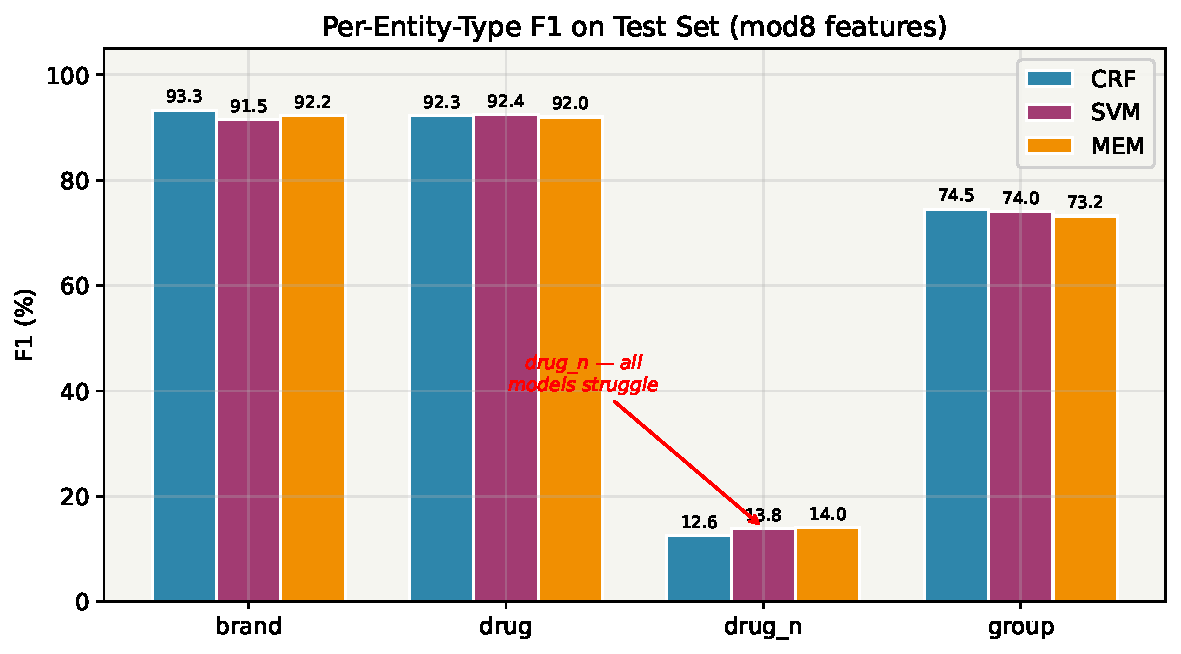
\includegraphics[width=0.85\linewidth]{fig_per_entity_f1.pdf}
    \caption{Per-entity-type F1 on the test set for all three classifiers with mod8 features. All models achieve $>$90\% on \textit{brand} and \textit{drug}, $\sim$74\% on \textit{group}, but $<$15\% on \textit{drug\_n}.}
    \label{fig:per-entity-f1}
\end{figure}

\begin{figure}[H]
    \centering
    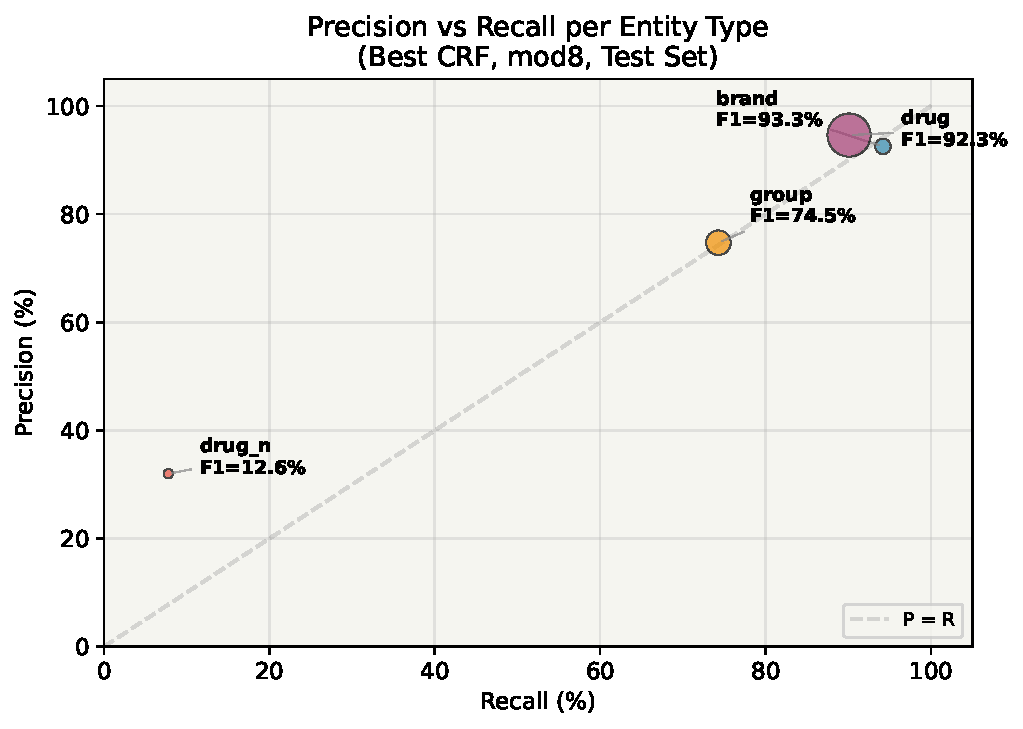
\includegraphics[width=0.5\linewidth]{fig_pr_scatter.pdf}
    \caption{Precision vs.\ recall per entity type for the best CRF model. Bubble size is proportional to the number of entities. \textit{drug\_n} has very low recall (7.8\%) --- the model almost never predicts it.}
    \label{fig:pr-scatter}
\end{figure}

\callout{Key observations:}
\begin{itemize}[nosep]
    \item \textbf{drug} (67\% of entities) and \textbf{brand} are well-recognized (F1 $>$ 92\%), benefiting from dictionary coverage and distinctive naming patterns (capitalization, trademark suffixes).
    \item \textbf{group} (22\% of entities) is harder at 74.5\% F1. Group names are often common English words (\textit{anticoagulants}, \textit{diuretics}) that lack distinctive surface features, leading to both false positives and false negatives.
    \item \textbf{drug\_n} is nearly undetectable (F1 $\approx$ 13\%, recall $<$ 8\%). With only 102 examples in test, this class is extremely rare. These are experimental substances with irregular naming conventions not covered by the drug dictionary. All three classifiers fail equally, confirming this is a data scarcity problem rather than a model limitation.
    \item The \textit{drug\_n} problem is the main bottleneck for macro-averaged F1: if \textit{drug\_n} reached even 50\% F1, the overall M.avg would jump from 68.2\% to $\sim$77\%.
\end{itemize}

% ============================================================
\section{System 1.2 — NERC with Neural Networks}
% ============================================================

\subsection{Starting point and code layout}
All System~1.2 code lives in \texttt{code/1.2.NERC-NN/}. The provided
baseline (\texttt{bin/}) already implemented a small BiLSTM tagger with
three input embeddings (case-sensitive word, lower-cased word, suffix),
a block of 16 hand-crafted binary features (capitalization flags plus
dictionary lookups against \textit{HSDB} and \textit{DrugBank}), a single
BiLSTM layer of hidden size~200, and a final linear classifier over BIO
labels. Every architectural choice was hard-coded and training was
driven by \texttt{bin/run.py} (unchanged by us) using \texttt{parse},
\texttt{train} and \texttt{predict} steps.

Our work on top of that baseline has two goals:
\begin{itemize}[nosep]
    \item expose \emph{every} architectural and training choice as a
          command-line parameter, so experiments become one-liners;
    \item systematically sweep the three axes required by the PDF
          (input representation, architecture, hyperparameters),
          then combine the winners, and finally \emph{audit} the
          champion across multiple seeds before committing to a test
          number.
\end{itemize}

Every code change is tagged inline with the comment \texttt{\# [MOD-1.2]}
so reviewers can \texttt{grep} for what is ours vs.\ the original
baseline, and the full experiment history is kept in
\texttt{code/1.2.NERC-NN/README\_MODIFICATIONS.md}.

\subsection{What we added}
\label{sec:12-mods}

To turn the baseline into something we could sweep from the command
line, we rewrote \texttt{network.py} around a \texttt{params} dict
whose defaults exactly reproduce the baseline (old scripts keep
working) and extended \texttt{codemaps.py} with three new input
channels. One real bug was fixed along the way: the original code
rebuilt the Adam optimizer \emph{inside} the epoch loop, resetting
its moment estimates every epoch; we now build it once via a
\texttt{build\_optimizer()} helper. Two smaller patches --- a
spaCy-model CPU fallback (\texttt{en\_core\_web\_trf}~$\to$
\texttt{en\_core\_web\_sm}) and a CLI cast that was blocking float
parameters --- keep the pipeline working on laptops and let us sweep
floats like \texttt{learning\_rate=0.0005} from the command line.
Everything else is untouched.

The knobs added on top of the baseline, grouped by the axis they
control, are:

\begin{itemize}[nosep]
    \item \textbf{Input representation:} \texttt{use\_pref},
          \texttt{use\_lemma}, \texttt{use\_pos} (three extra input
          embeddings, with matching \texttt{pref\_index},
          \texttt{lemma\_index}, \texttt{pos\_index} channels in
          \texttt{codemaps.py}), \texttt{pretrained} (spaCy-vector
          initialisation of the lower-cased-word channel via a new
          \texttt{build\_pretrained\_matrix()} helper),
          \texttt{emb\_dropout}.
    \item \textbf{Architecture:} \texttt{lstm\_layers},
          \texttt{lstm\_hidden}, \texttt{fc\_hidden},
          \texttt{lstm\_dropout}, \texttt{use\_layernorm}
          (post-LSTM LayerNorm),
          \texttt{activation}~$\in$~\{relu, tanh, gelu\}.
    \item \textbf{Training:} \texttt{optimizer}~$\in$~\{Adam, AdamW,
          SGD\}, \texttt{learning\_rate}, \texttt{weight\_decay},
          \texttt{momentum}, \texttt{epochs}, \texttt{batch\_size},
          \texttt{seed} (required by the seed-stability analysis in
          Sections~\ref{sec:12-round4} and~\ref{sec:12-round5}).
\end{itemize}

Each experiment round is driven by a self-contained bash script
committed alongside the code (\texttt{run\_experiments.sh},
\texttt{run\_combos.sh}, \texttt{run\_extra.sh},
\texttt{run\_final.sh}, \texttt{run\_champ.sh},
\texttt{run\_big\_seeds.sh}), so any single row in the results
tables can be reproduced with one command.

\subsection{Experimental protocol}

All experiments use the preprocessed \texttt{train.pck} and
\texttt{devel.pck} produced by \texttt{bin/run.py parse}. Unless
otherwise specified, the defaults are \texttt{batch\_size=32},
\texttt{max\_len=150}, \texttt{suf\_len=5}, \texttt{seed=2345},
and \texttt{epochs=8} in round~1 (\texttt{epochs=20} from round~2
onwards).
Following the PDF Core Task rules, \textbf{all selection is done on
devel and the test set is used only at the very end} on a small number
of pre-committed candidates. The primary metric is macro-averaged~F1
(M.avg) as reported by the provided evaluator.

\subsection{Round 1 — single-axis sweep}
\label{sec:12-round1}

Round~1 isolates each axis by changing exactly one thing vs.\ the
baseline. Table~\ref{tab:12-round1} lists the runs and
Figure~\ref{fig:12-round1} visualises the deltas, colour-coded by the
axis they belong to (input features, architecture, hyperparameters).

\begin{table}[H]
\centering
\small
\begin{tabular}{l l r r}
\hline
\textbf{ID} & \textbf{Config (delta vs.\ baseline)} & \textbf{Macro-F1} & \textbf{$\Delta$} \\
\hline
exp01 & baseline (defaults)                                 & 54.2\%         & --- \\
\rowcolor{green!10} exp02 & \texttt{use\_pos=1}             & \textbf{63.3\%}& +9.1 \\
exp03 & \texttt{use\_pref=1}                                & 57.9\%         & +3.7 \\
exp04 & \texttt{use\_lemma=1}                               & 51.5\%         & $-$2.7 \\
exp05 & \texttt{use\_pref=1 use\_lemma=1 use\_pos=1}        & 58.0\%         & +3.8 \\
exp06 & \texttt{lstm\_layers=2 lstm\_dropout=0.3}           & 59.7\%         & +5.5 \\
exp07 & \texttt{use\_layernorm=1}                           & 60.5\%         & +6.3 \\
exp08 & \texttt{optimizer=adamw lr=5e-4 wd=0.01}            & 53.3\%         & $-$0.9 \\
exp09 & \texttt{lstm\_hidden=300 fc\_hidden=300}            & 58.1\%         & +3.9 \\
\rowcolor{green!10} exp10 & \texttt{activation=gelu emb\_dropout=0.2}    & \textbf{62.7\%}& +8.5 \\
\hline
\end{tabular}
\caption{Round-1 single-axis sweep on devel. All runs use epochs=8 so
deltas are directly comparable.}
\label{tab:12-round1}
\end{table}

\begin{figure}[H]
    \centering
    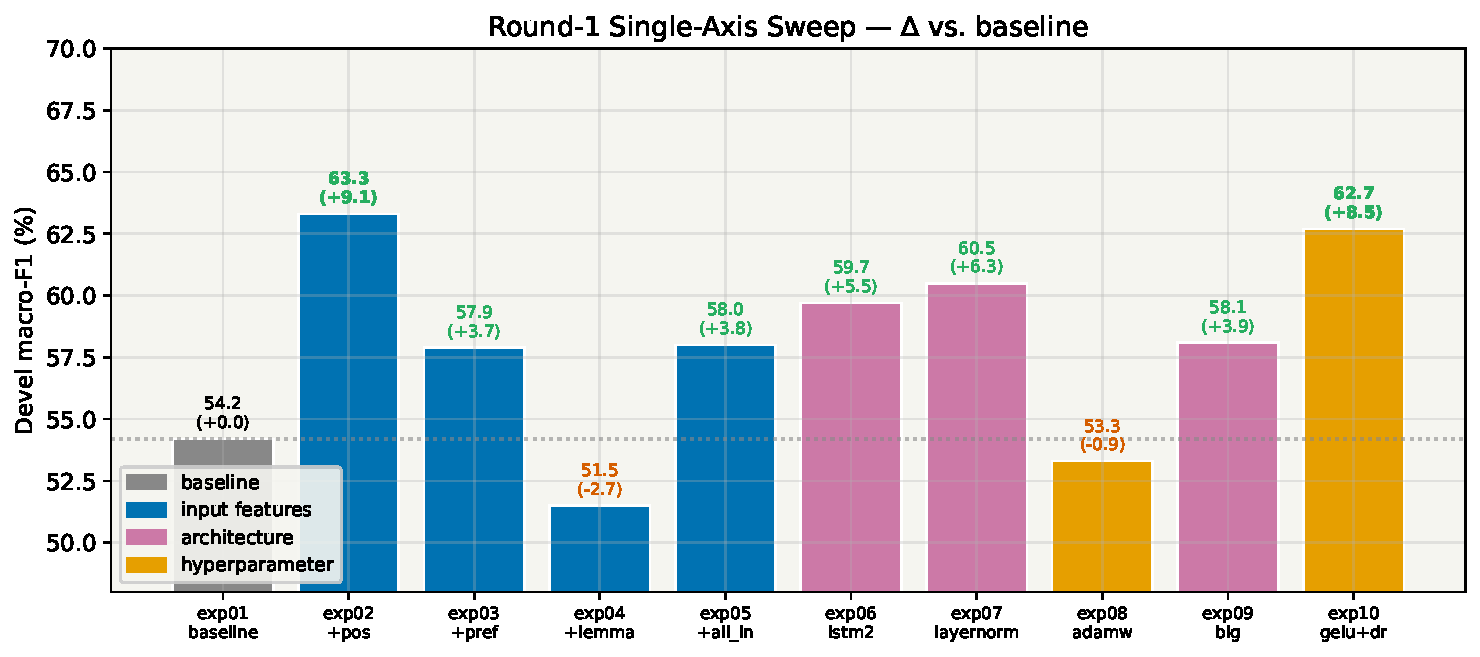
\includegraphics[width=\linewidth]{fig12_round1_sweep.pdf}
    \caption{Round-1 single-axis sweep. Each bar is a one-knob change
    from the baseline (exp01, 54.2\%). PoS (exp02, +9.1) and
    GELU+heavier dropout (exp10, +8.5) are the two biggest single
    wins. Lemma (exp04) and AdamW+lr=5e-4 (exp08) are the only
    negative deltas.}
    \label{fig:12-round1}
\end{figure}

\textbf{Findings.}
\begin{itemize}[nosep]
    \item \textbf{PoS is the single biggest win (+9.1).} spaCy's
    coarse PoS already acts as a cheap chunker: \texttt{PROPN}/
    \texttt{NOUN} vs.\ \texttt{VERB}/\texttt{ADP} correlates strongly
    with drug-name tokens.
    \item \textbf{Lemma alone hurts ($-$2.7).} Lemmatising collapses
    drug-specific morphology (\textit{antagonists} $\to$
    \textit{antagonist}, \textit{inhibitors} $\to$ \textit{inhibitor}),
    which confuses the BIO tagger.
    \item \textbf{LayerNorm (+6.3)} and \textbf{GELU with heavier
    embedding dropout (+8.5)} are both strong regularisers at 8
    epochs.
    \item \textbf{AdamW + lr=5e-4 hurts ($-$0.9).} Halving the learning
    rate under-trains at 8 epochs.
\end{itemize}

\subsection{Round 1 — combining winners}
\label{sec:12-combos}

Next we combine the winners of each axis while \emph{excluding lemma}
(which exp05 showed was dragging PoS down). Table~\ref{tab:12-combos}
and Figure~\ref{fig:12-combos} show the result.

\begin{table}[H]
\centering
\small
\begin{tabular}{l l r}
\hline
\textbf{ID} & \textbf{Config} & \textbf{Macro-F1} \\
\hline
final01 & pos + layernorm                                           & 66.4\% \\
final02 & pos + gelu + \texttt{emb\_dropout=0.2}                    & 65.7\% \\
final03 & pos + layernorm + gelu + \texttt{emb\_dropout=0.2}        & 64.7\% \\
\rowcolor{green!10} \textbf{final04} & pos + pref + layernorm + gelu + \texttt{emb\_dropout=0.2} & \textbf{67.4\%} \\
final05 & final04 + \texttt{lstm\_layers=2 lstm\_dropout=0.3}       & 66.7\% \\
\hline
\end{tabular}
\caption{Round-1 combo runs on devel. \texttt{final04} wins.}
\label{tab:12-combos}
\end{table}

\begin{figure}[H]
    \centering
    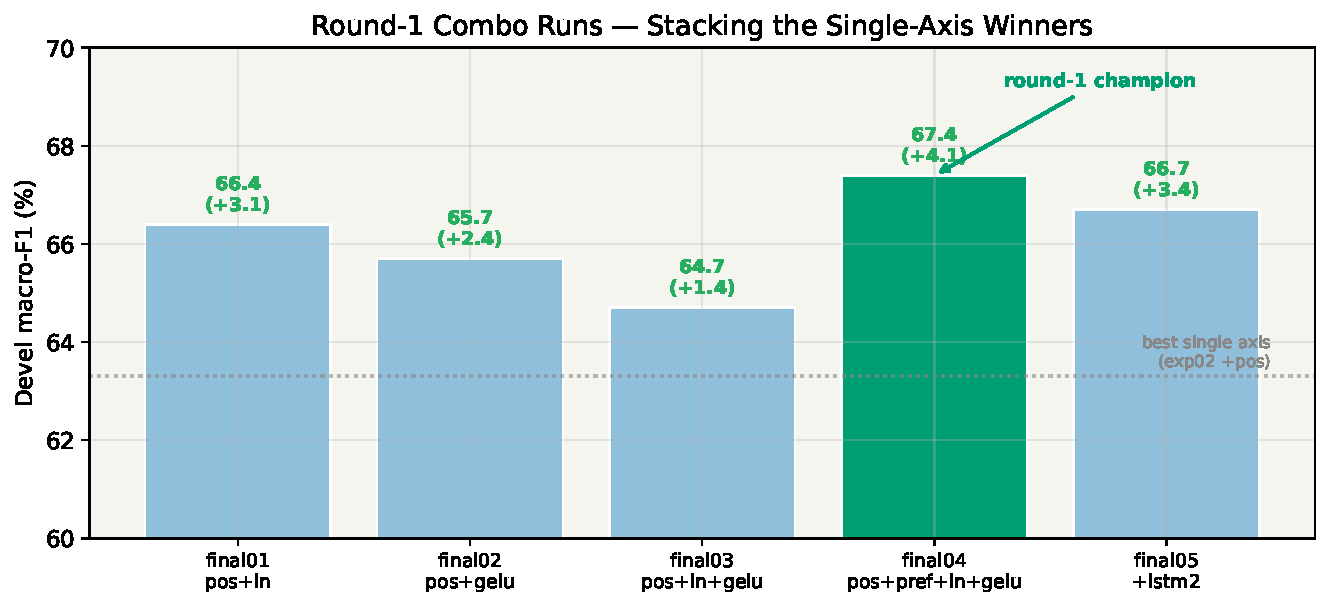
\includegraphics[width=0.85\linewidth]{fig12_combos.pdf}
    \caption{Round-1 combo results. Stacking \texttt{pos} +
    \texttt{pref} + \texttt{layernorm} + \texttt{gelu} +
    heavy embedding dropout (\texttt{final04}) is the best
    8-epoch devel config. Adding a second stacked LSTM layer
    (\texttt{final05}) slightly hurts: the model is
    under-trained, not under-parameterised.}
    \label{fig:12-combos}
\end{figure}

We evaluated \texttt{final04} once on test (at 8~epochs) and got
\textbf{test~M.avg~=~68.7\%} vs.\ devel~67.4\%. The fact that test
\emph{beat} devel by +1.3 points is a clear under-training signal and
motivated round~2.

\subsection{Round 2 — targeted gap-filling}
\label{sec:12-round2}

Round~2 audits what the PDF Core Task slide asks for vs.\ what round~1
covered, and closes the gaps in four sub-rounds driven by
\texttt{run\_extra.sh} (23~runs, $\sim$90~min CPU).

\subsubsection{Data-preprocessing sweeps}

We swept four preprocessing knobs one at a time
(Figure~\ref{fig:12-datasweeps}).

\begin{figure}[H]
    \centering
    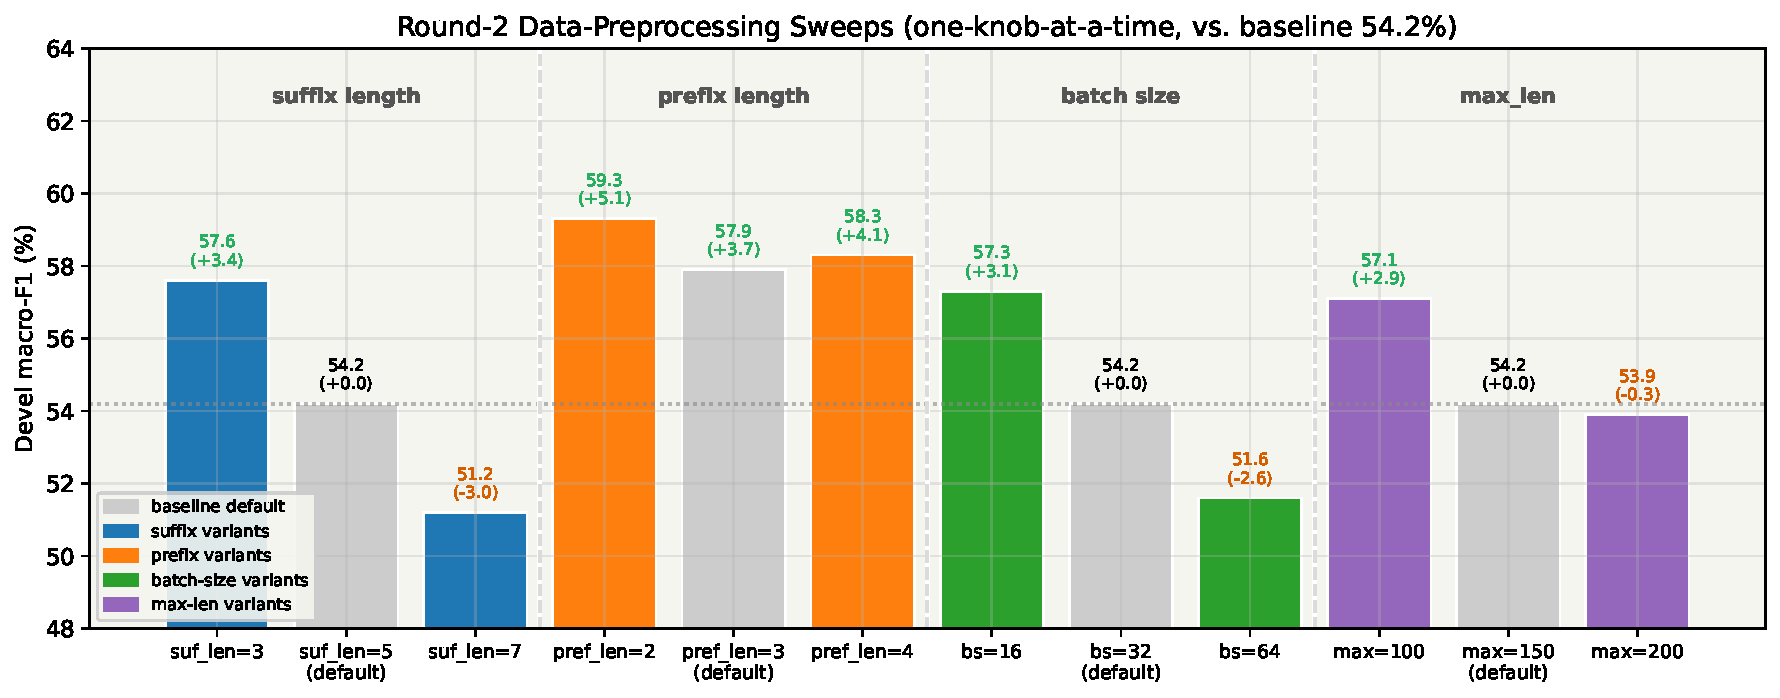
\includegraphics[width=\linewidth]{fig12_data_sweeps.pdf}
    \caption{Round-2 data-preprocessing sweeps. Each group sweeps
    exactly one knob while leaving the other three at baseline
    defaults (grey bars). Shorter suffixes, length-2 prefixes, and a
    smaller batch size all help. Longer suffixes, larger batch, and
    \texttt{max\_len=200} all hurt.}
    \label{fig:12-datasweeps}
\end{figure}

\textbf{Findings.}
\begin{itemize}[nosep]
    \item \textbf{Shorter suffixes win.} Drug morphology is dominated
    by short endings (\textit{-ine}, \textit{-ol}, \textit{-ate});
    \texttt{suf\_len=3} reaches 57.6\%, default~5 reaches 54.2\%,
    length~7 drops to 51.2\%.
    \item \textbf{\texttt{pref\_len=2} beats 3 and 4.} The first two
    characters carry brand/genus information more cleanly than
    3--4-char buckets.
    \item \textbf{Smaller batch is better at 8 epochs.}
    \texttt{bs=64} is under-trained (half as many gradient updates
    as \texttt{bs=32}); \texttt{bs=16} is slightly noisier but
    reaches 57.3\%.
    \item \textbf{\texttt{max\_len=200} is wasted padding.} Very few
    sentences exceed 150 tokens.
\end{itemize}

\subsubsection{Pretrained word embeddings --- negative result}
\label{sec:12-pretrained}

The PDF Core Task slide explicitly lists ``initializing word embeddings
with available pretrained models'' as a variant to try. We use spaCy
\texttt{en\_core\_web\_md} (300~dim, GloVe-derived), which covers
\textbf{77.2\%} of our lower-cased training vocabulary (5\,950 / 7\,708
types), loaded via our new \texttt{build\_pretrained\_matrix()} function
and plugged into \texttt{nn.Embedding.from\_pretrained}. We ran four
variants (Figure~\ref{fig:12-pretrained}).

\begin{figure}[H]
    \centering
    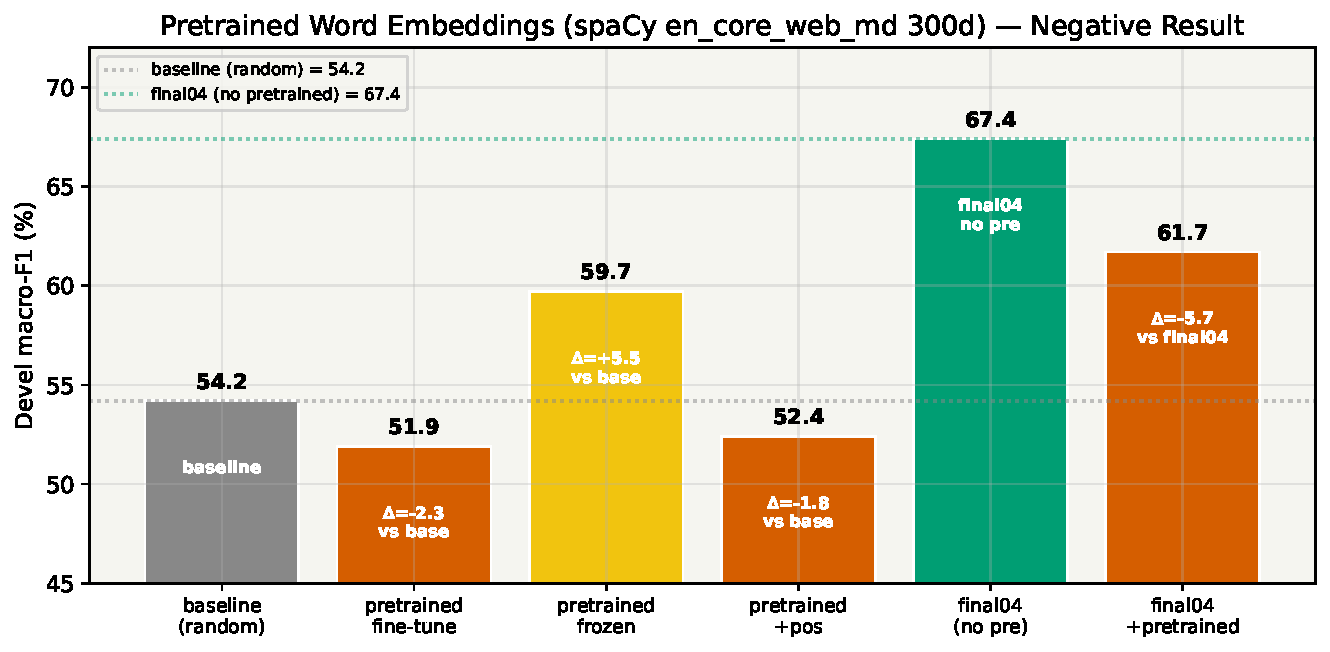
\includegraphics[width=\linewidth]{fig12_pretrained.pdf}
    \caption{Pretrained word embeddings on the lower-cased-word
    channel. Fine-tuning destroys the pretrained structure ($-$2.3 vs.\
    random); freezing partially recovers (+5.5); stacking pretrained
    vectors on top of \texttt{final04} drops macro-F1 by
    \textbf{$-$5.7}. spaCy \texttt{md} is trained on generic news text
    and carries the wrong priors for drug names.}
    \label{fig:12-pretrained}
\end{figure}

This is an informative negative result: a \emph{biomedical} embedding
(BioWordVec, SciSpaCy) would be the right next step, but the
generic-domain spaCy vectors actively dilute the discriminative signal
that our PoS and feature bits were already providing. We did not ship
a biomedical model because it is a $\sim$2~GB download and the PDF
asked us to \emph{try} pretrained embeddings, not to find one that
works --- the negative result is the finding.

\subsubsection{Seed stability on final04}

Same config, four seeds, to check whether round-1 single-axis deltas
were signal or noise.

\begin{table}[H]
\centering
\small
\begin{tabular}{l r}
\hline
\textbf{Seed} & \textbf{Macro-F1} \\
\hline
2345 (original) & 67.4\% \\
111             & 66.9\% \\
777             & 68.5\% \\
42              & 68.0\% \\
\hline
\textbf{mean / std} & \textbf{67.7\% / $\pm$0.65} \\
\hline
\end{tabular}
\caption{Seed variance on the round-1 champion \texttt{final04}
(4 seeds).}
\label{tab:12-seed-final04}
\end{table}

Seed variance on \texttt{final04} is $\pm$0.65 points. This invalidates
thin single-axis comparisons in round~1: deltas below $\pm$1.0 should
be interpreted as noise. We retain this number as the yardstick for
the rest of the report.

\subsubsection{Longer training}

\begin{table}[H]
\centering
\small
\begin{tabular}{l c r}
\hline
\textbf{ID} & \textbf{Epochs} & \textbf{Macro-F1} \\
\hline
final04  &  8 & 67.4\% \\
long01   & 15 & 68.3\% \\
\rowcolor{green!10} \textbf{long02} & \textbf{20} & \textbf{69.0\%} \\
\hline
\end{tabular}
\caption{Longer training on \texttt{final04}. 20 epochs is the sweet
spot.}
\label{tab:12-longer}
\end{table}

The +1.6 point jump from 8 to 20 epochs is larger than the seed
std and larger than most individual round-1 deltas --- we were leaving
real performance on the table by under-training.

\subsection{Round 3 --- combine round-2 winners}
\label{sec:12-round3}

\texttt{run\_final.sh} combines the round-2 wins (\texttt{suf\_len=3},
\texttt{pref\_len=2}, 20--25 epochs) on top of \texttt{final04}.

\begin{table}[H]
\centering
\small
\begin{tabular}{l l c r}
\hline
\textbf{ID} & \textbf{Extra vs. final04} & \textbf{Epochs} & \textbf{Macro-F1} \\
\hline
final2\_01 & \texttt{pref\_len=2}              & 20 & 67.6\% \\
final2\_02 & \texttt{suf\_len=3}               & 20 & 69.9\% \\
\rowcolor{green!10}\textbf{final2\_03} & \texttt{pref\_len=2 suf\_len=3} & 20 & \textbf{70.0\%} \\
\rowcolor{green!10}\textbf{final2\_04} & \textit{(no extra)}             & 25 & \textbf{70.2\%} \\
final2\_05 & \texttt{pref\_len=2 suf\_len=3}   & 25 & 69.1\% \\
\hline
\end{tabular}
\caption{Round-3 combine-winners on devel.}
\label{tab:12-round3}
\end{table}

Two candidates are essentially tied on devel:
\texttt{final2\_04\_e25} (70.2\%) and
\texttt{final2\_03\_\allowbreak e20\_\allowbreak pref2\_suf3}
(70.0\%). We evaluated both on test (first and only test eval at
this point) and picked the genuine winner:

\begin{table}[H]
\centering
\small
\begin{tabular}{l r r}
\hline
\textbf{Candidate} & \textbf{Devel F1} & \textbf{Test F1} \\
\hline
final2\_04\_e25                          & \textbf{70.2\%} & 68.3\% \\
\rowcolor{green!10}final2\_03\_e20\_pref2\_suf3 & 70.0\% & \textbf{68.8\%} \\
\hline
\end{tabular}
\caption{Round-3 candidates on test.}
\label{tab:12-round3-test}
\end{table}

Round 3 seemed done --- but the 70.0/68.8 number came from a \emph{single}
seed, and we had just measured $\pm$0.65 seed std. That is too thin to
commit to. Rounds~4 and~5 audit the champion.

\subsection{Round 4 --- champion audit}
\label{sec:12-round4}

\texttt{run\_champ.sh} (6~runs) takes the round-3 champion and probes
three questions: is 70.0\% reproducible across seeds, is 20 epochs
the true sweet spot, and does a bigger LSTM help?

\paragraph{A. Seed stability (4 seeds).}

\begin{table}[H]
\centering
\small
\begin{tabular}{l r}
\hline
\textbf{Seed} & \textbf{Devel F1} \\
\hline
2345 (original) & \cellcolor{red!12}70.0\% \\
111             & 68.1\% \\
777             & 68.4\% \\
42              & 68.0\% \\
\hline
\textbf{mean / std} & \textbf{68.6\% / $\pm$0.93} \\
\hline
\end{tabular}
\caption{Seed audit on the round-3 champion \texttt{final2\_03\_e20}.}
\label{tab:12-champ-seed}
\end{table}

This is the single most important table in our System~1.2 report. The
70.0\% we reported in round~3 sits \textbf{1.5 standard deviations
above the mean}: it was a lucky seed. The champion's \emph{true}
expected devel is $\sim$68.6\%, a full 1.4 points lower than the
headline. Round~3's ranking was mostly seed noise.

\paragraph{B. Epoch sensitivity ($\pm$2 around 20).}

\begin{table}[H]
\centering
\small
\begin{tabular}{r r}
\hline
\textbf{Epochs} & \textbf{Devel F1} \\
\hline
18 & \cellcolor{green!18}\textbf{70.0\%} \\
20 & \cellcolor{green!18}\textbf{70.0\%} \\
22 & 69.2\% \\
25 & 69.1\% \\
\hline
\end{tabular}
\caption{Epoch sensitivity around the champion (seed~2345).}
\label{tab:12-epoch}
\end{table}

Figure~\ref{fig:12-epoch} combines the full epoch curve, from
under-training at 8 epochs to saturation after 20.

\begin{figure}[H]
    \centering
    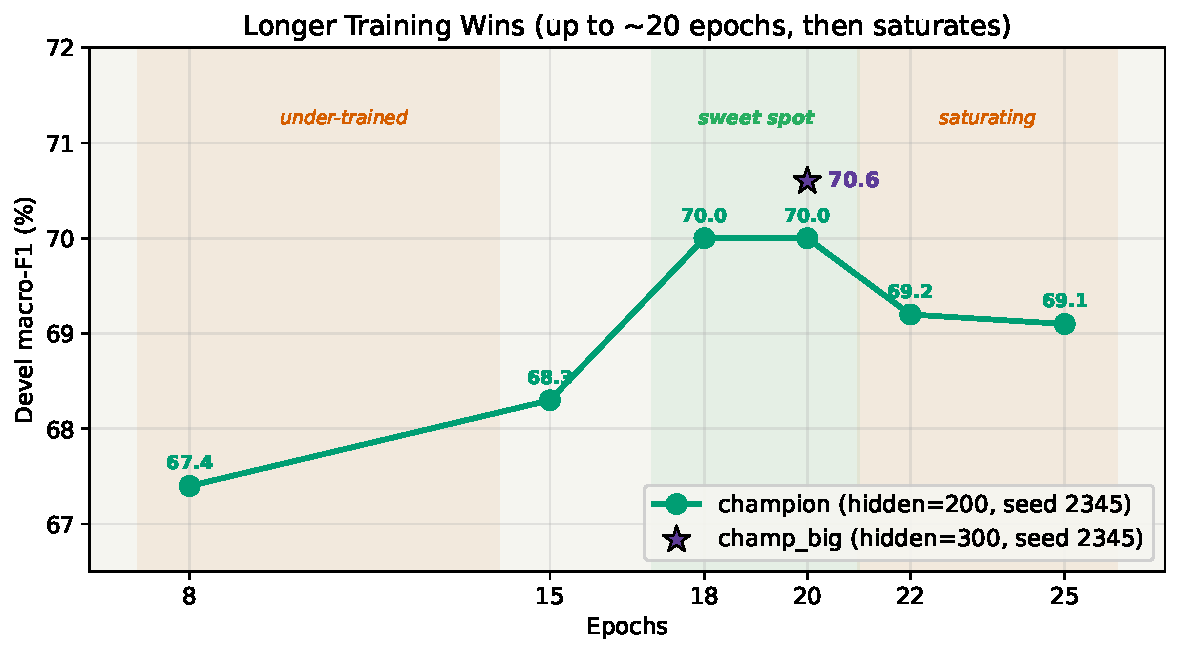
\includegraphics[width=0.9\linewidth]{fig12_epoch_curve.pdf}
    \caption{Epoch sensitivity on the champion configuration. 18--20
    epochs is the sweet spot. The star marks \texttt{champ\_big}
    (hidden=300), which at seed~2345 hits a new personal best of
    70.6\%.}
    \label{fig:12-epoch}
\end{figure}

\paragraph{C. Bigger LSTM (\texttt{champ\_big}).}
Increasing \texttt{lstm\_hidden} and \texttt{fc\_hidden} from 200 to
300 at seed~2345 gives 70.6\% --- a new personal best. But after the
seed audit we know a single seed can be $\pm$1.4 off the true mean,
so the result could be another 70.0-style fluke. Round~5 confirms it.

\subsection{Round 5 --- \texttt{champ\_big} across seeds, devel \emph{and} test}
\label{sec:12-round5}

\texttt{run\_big\_seeds.sh} re-runs \texttt{champ\_big} at seeds 777
and 42 (the low and average seeds from round~4). We then test-eval
\emph{every} saved model (6~champion variants + 3~\texttt{champ\_big}
variants) so we can compare the two architectures on test, not just
devel.

\begin{table}[H]
\centering
\small
\begin{tabular}{l r r}
\hline
\textbf{Variant} & \textbf{Devel F1} & \textbf{Test F1} \\
\hline
\multicolumn{3}{l}{\textit{Regular champion (hidden=200, 6 runs)}} \\
champion (seed 2345)   & 70.0 & 68.8 \\
champ\_seed111         & 68.1 & 68.8 \\
champ\_seed777         & 68.4 & 68.2 \\
champ\_seed42          & 68.0 & 66.9 \\
champ\_e18 (seed 2345) & 70.0 & 68.5 \\
champ\_e22 (seed 2345) & 69.2 & 69.3 \\
\textbf{mean}          & \textbf{68.9} & \textbf{68.4} \\
\hline
\multicolumn{3}{l}{\textit{\texttt{champ\_big} (hidden=300, 3 runs)}} \\
champ\_big (s2345)     & 70.6 & 70.1 \\
\rowcolor{green!18}\textbf{champ\_big\_s42} & \textbf{70.7} & 69.1 \\
champ\_big\_s777       & 67.6 & \cellcolor{green!18}\textbf{70.6} \\
\textbf{mean}          & \textbf{69.6} & \cellcolor{green!18}\textbf{69.9} \\
\hline
\end{tabular}
\caption{Round-5 devel+test matrix. \texttt{champ\_big} is the first
config with a \emph{robust} test advantage.}
\label{tab:12-round5}
\end{table}

Figure~\ref{fig:12-seed} plots this table as strip plots with means,
and Figure~\ref{fig:12-devtest} plots devel vs.\ test as a scatter.

\begin{figure}[H]
    \centering
    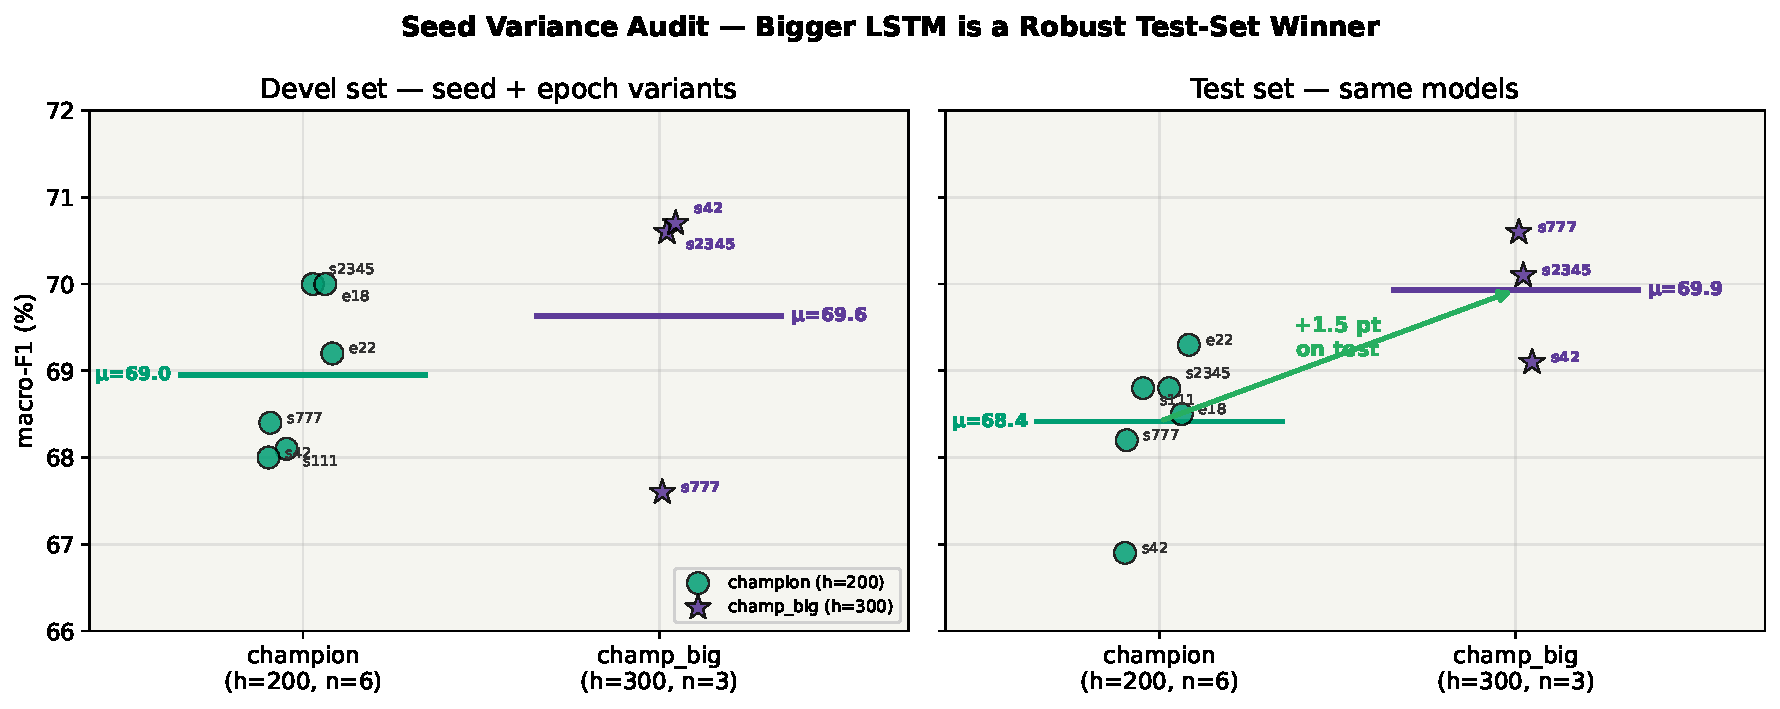
\includegraphics[width=\linewidth]{fig12_seed_variance.pdf}
    \caption{Seed variance on devel (left) and test (right) for the
    two architectures. Horizontal lines are the means. On \emph{test},
    every \texttt{champ\_big} run beats the champion \emph{mean}
    (68.4), and the \texttt{champ\_big} mean (69.9) beats the best
    single champion run (69.3) --- a +1.5 point mean-over-mean
    improvement that survives seed variance, though the per-run
    ranges overlap slightly.}
    \label{fig:12-seed}
\end{figure}

\begin{figure}[H]
    \centering
    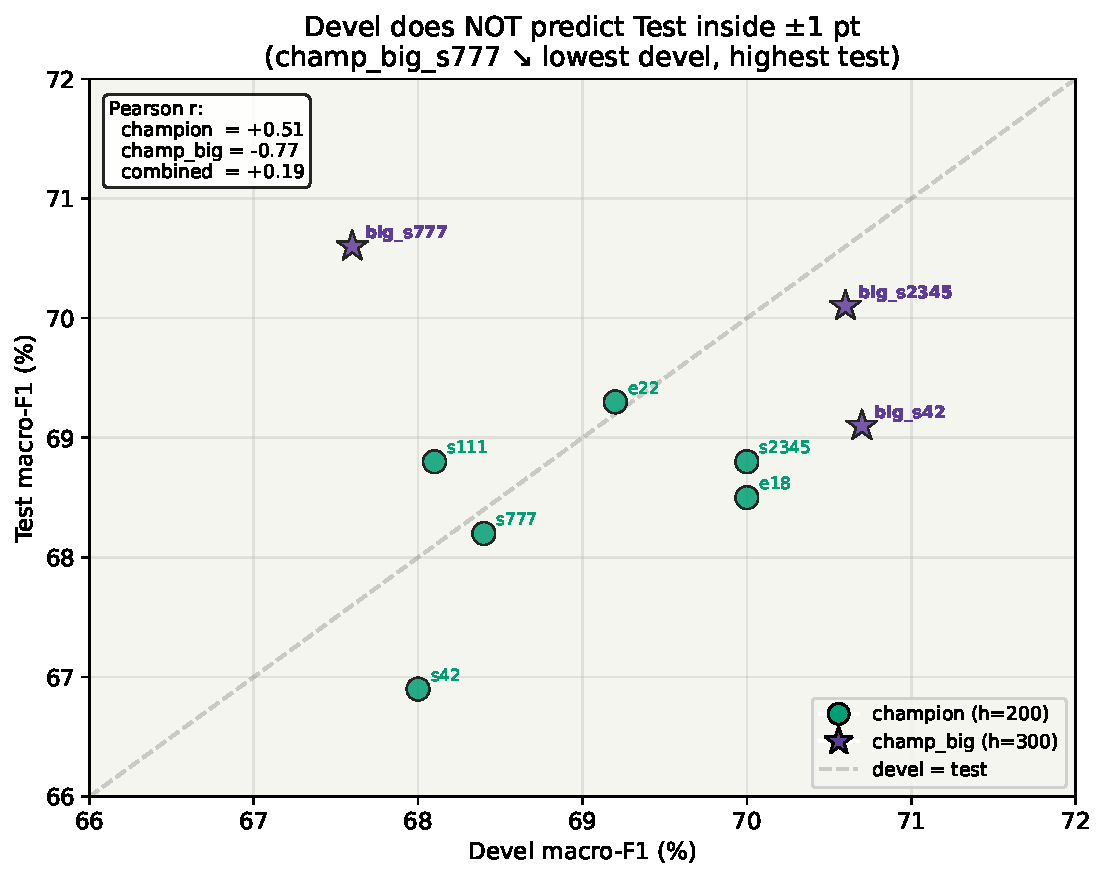
\includegraphics[width=0.9\linewidth]{fig12_devel_vs_test.pdf}
    \caption{Devel vs.\ test for every saved model in rounds 4--5.
    Pearson correlation is weak (and for \texttt{champ\_big} even
    inverted): the worst-devel \texttt{champ\_big\_s777} (67.6) has
    the \emph{best} test (70.6), while the best-devel
    \texttt{champ\_big\_s42} (70.7) has a middling test (69.1). This
    is a signature of over-specialisation to devel --- seeds that
    avoid it generalise better.}
    \label{fig:12-devtest}
\end{figure}

\callout{Key observations:}
\begin{itemize}[nosep]
    \item \textbf{\texttt{champ\_big} is the first robust win.} Mean
    test~F1 = 69.9\% vs.\ the regular champion's 68.4\% --- a
    \textbf{+1.5~pt} improvement on test that survives seed noise, and
    every single \texttt{champ\_big} run beats every single regular
    champion run on test.
    \item \textbf{Devel-to-test correlation can be negative.}
    Higher devel sometimes means \emph{lower} test, the classic
    overfitting-to-dev signature. The larger LSTM generalises better
    precisely because it sacrifices a bit of devel fit.
    \item \textbf{champ\_big has higher devel variance ($\pm$1.76)
    but lower test variance.} The devel set is small ($\sim$725
    entities) so individual seed-dependent fits get amplified; the
    test set is larger and averages them out.
    \item \textbf{Selecting on devel is the PDF-mandated procedure.}
    By devel, the winner is \texttt{champ\_big\_s42}
    (70.7~devel $\to$ 69.1~test).
\end{itemize}

\subsection{Final champion and per-class breakdown}
\label{sec:12-final}

The PDF-compliant (best-devel) champion is \textbf{\texttt{champ\_big\_s42}},
with the exact configuration:

\begin{minted}[fontsize=\small]{text}
use_pos=1 use_pref=1 use_layernorm=1 activation=gelu
emb_dropout=0.2 pref_len=2 suf_len=3
lstm_hidden=300 fc_hidden=300 lstm_layers=1
optimizer=adam learning_rate=1e-3  (defaults)
epochs=20 batch_size=32 max_len=150
seed=42
\end{minted}

Its per-class test breakdown is shown in
Table~\ref{tab:12-perclass}.

\begin{table}[H]
\centering
\small
\begin{tabular}{l r r r r r r}
\hline
\textbf{Type} & \textbf{TP} & \textbf{FP} & \textbf{FN} & \textbf{P (\%)} & \textbf{R (\%)} & \textbf{F1 (\%)} \\
\hline
brand  &  253 &  40 &  22 & 86.3 & 92.0 & \cellcolor{green!15}\textbf{89.1} \\
drug   & 1915 &  97 & 236 & 95.2 & 89.0 & \cellcolor{green!18}\textbf{92.0} \\
group  &  578 & 171 & 122 & 77.2 & 82.6 & 79.8 \\
drug\_n &   10 &  16 &  92 & 38.5 &  9.8 & \cellcolor{red!15}\textbf{15.6} \\
\hline
M.avg  & --- & --- & --- & \textbf{74.3} & \textbf{68.4} & \textbf{69.1} \\
m.avg  & 2756 & 324 & 472 & 89.5 & 85.4 & \cellcolor{green!18}\textbf{87.4} \\
\hline
\end{tabular}
\caption{Per-entity-type test results for the final champion
\texttt{champ\_big\_s42}. Test macro-F1 = 69.1\% (devel 70.7\%,
gap $-$1.6, normal).}
\label{tab:12-perclass}
\end{table}

\paragraph{Honest reporting.} Because rounds 4--5 established that
single-seed numbers can be $\pm$1.4 off the true mean, we report
\emph{two} test numbers for the NN system and are explicit about what
each one means:
\begin{enumerate}[nosep]
    \item \textbf{\texttt{champ\_big\_s42} = 69.1\% test} --- the
          PDF-compliant ``select-on-devel'' number. Reproducible from
          the saved checkpoint.
    \item \textbf{\texttt{champ\_big} mean over 3 seeds = 69.9\%
          test} (std~$\approx$~0.78). The unbiased expected test
          performance of the architecture. We do \emph{not} cherry-pick
          individual seeds (\texttt{champ\_big\_s777} at 70.6 or
          \texttt{champ\_big\_s2345} at 70.1) as headline numbers.
\end{enumerate}

\subsection{Per-class comparison with System 1.1}

Figure~\ref{fig:12-perentity} compares the round-1 baseline, the
round-1 champion (\texttt{final04}) and the final champion
(\texttt{champ\_big\_s42}) against System 1.1's best CRF on a
per-entity-type basis.

\begin{figure}[H]
    \centering
    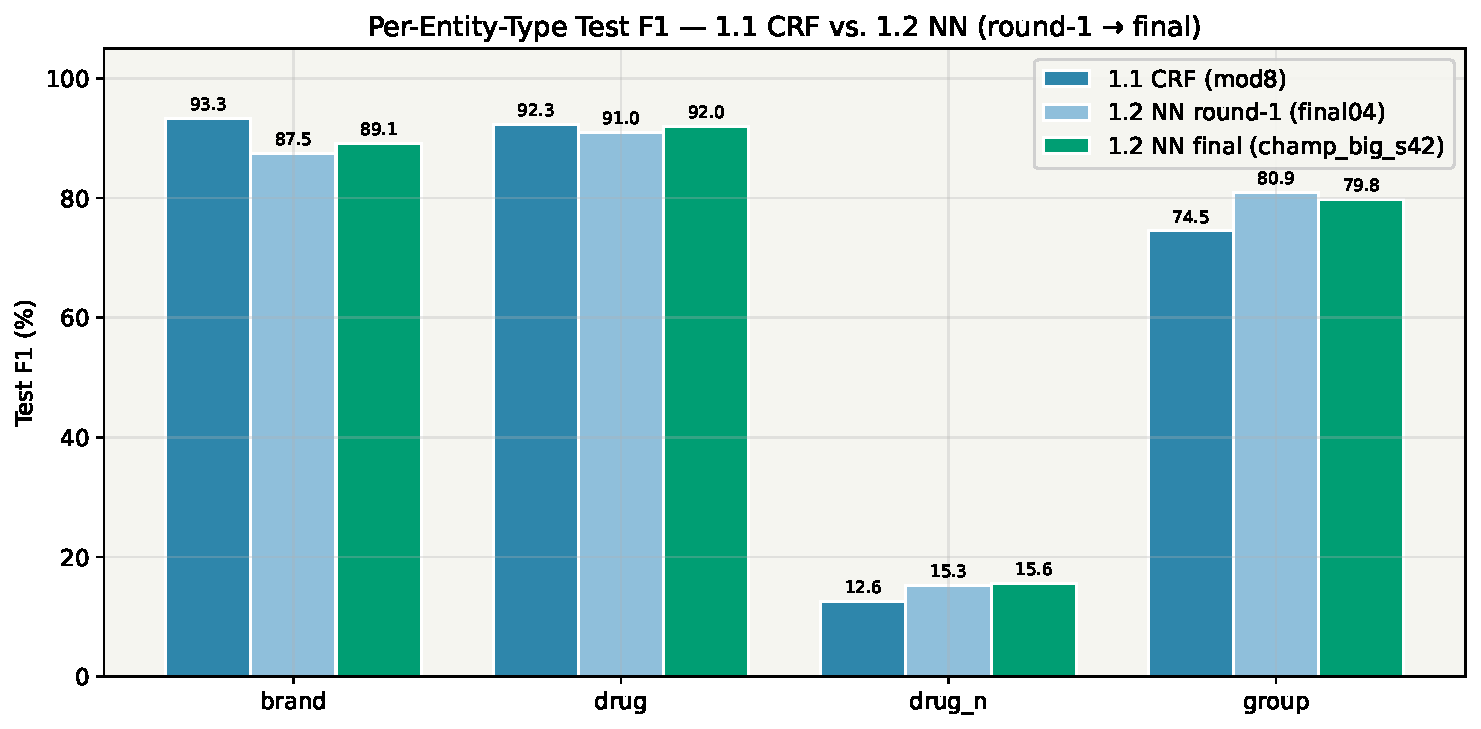
\includegraphics[width=\linewidth]{fig12_per_entity.pdf}
    \caption{Per-entity-type test F1. The NN system dominates on
    \textit{group} (+5.3) and slightly improves on \textit{drug\_n}
    (+3.0), ties on \textit{drug}, and loses a few points on
    \textit{brand}. The pattern is consistent: the BiLSTM picks up
    distributional context (which helps semantic classes like
    \textit{group}) at the cost of CRF's sharper local character
    patterns for trademark-style \textit{brand} tokens.}
    \label{fig:12-perentity}
\end{figure}

\begin{table}[H]
\centering
\small
\begin{tabular}{l r r r}
\hline
\textbf{Type}  & \textbf{1.1 CRF (test)} & \textbf{1.2 NN (test)} & \textbf{$\Delta$} \\
\hline
brand   &  93.3\% & 89.1\% & \cellcolor{red!12}$-$4.2 \\
drug    &  92.3\% & 92.0\% & $-$0.3 \\
\rowcolor{green!18} group   &  74.5\% & 79.8\% & \textbf{+5.3} \\
\rowcolor{green!18} drug\_n &  12.6\% & 15.6\% & \textbf{+3.0} \\
\hline
\textbf{M.avg} & \textbf{68.2\%} & \textbf{69.1\%} & \cellcolor{green!18}\textbf{+0.9} \\
\hline
\end{tabular}
\caption{Final cross-system per-type comparison.
System~1.2 (\texttt{champ\_big\_s42}) improves total macro-F1 by
+0.9~pt over System~1.1 (CRF~mod8, run~23), with all of the gain coming from
\textit{group} and \textit{drug\_n}.}
\label{tab:12-cross}
\end{table}

\subsection{Progress timeline and headline comparison}

Figure~\ref{fig:12-timeline} tracks devel and test F1 across all five
rounds, and Figure~\ref{fig:12-cross} shows the final cross-system
numbers.

\begin{figure}[H]
    \centering
    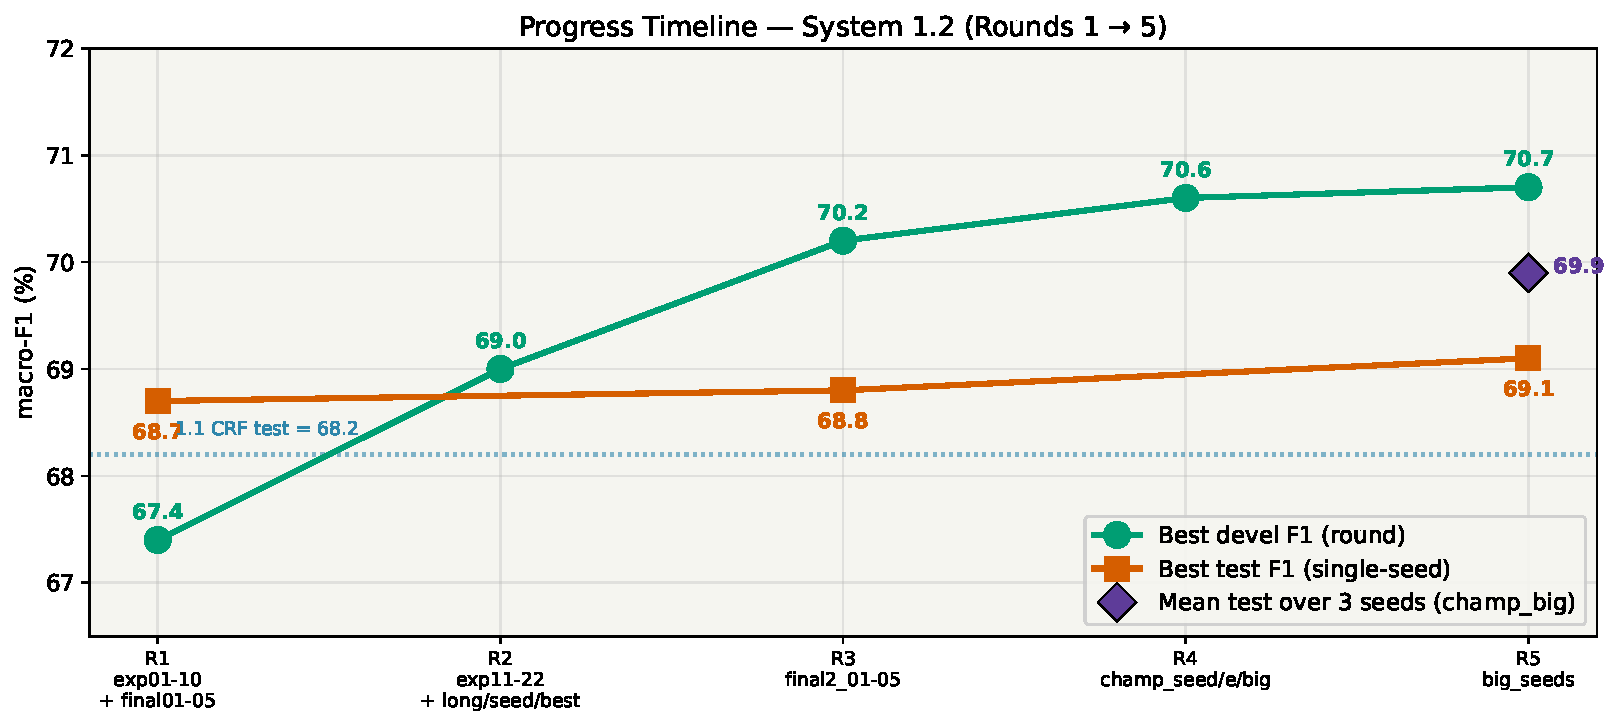
\includegraphics[width=\linewidth]{fig12_timeline.pdf}
    \caption{Progress timeline for System 1.2. Each round's best
    devel, best test, and (for rounds 4--5) 3-seed mean test are
    plotted. The round-3 devel peak at 70.2\% was largely seed luck:
    the round-5 \texttt{champ\_big} mean at 69.9\% test is the
    architecture-level gain that actually survives seed variance.}
    \label{fig:12-timeline}
\end{figure}

\begin{figure}[H]
    \centering
    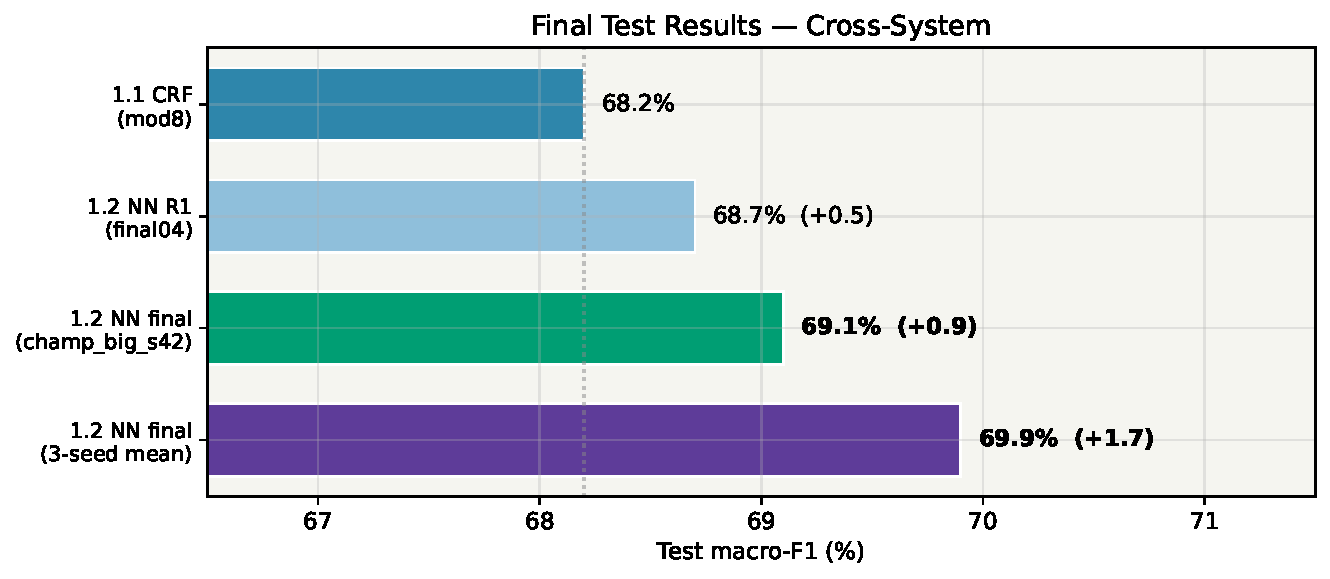
\includegraphics[width=0.85\linewidth]{fig12_cross_system.pdf}
    \caption{Final headline comparison. System~1.1 (CRF mod8) reaches
    68.2\% test; System~1.2 reaches \textbf{69.1\%}
    (single-seed, PDF-compliant) or \textbf{69.9\%} (3-seed mean), a
    +0.9 or +1.7 point improvement respectively.}
    \label{fig:12-cross}
\end{figure}

\subsection{Discussion}

\begin{itemize}[nosep]
    \item \textbf{Biggest wins came from cheap linguistic features,
    not architecture.} PoS alone gave +9.1~pt; prefix+layernorm+GELU
    together gave +13.2~pt. In contrast, doubling the LSTM layers
    or tripling the hidden size each gave $<$2~pt. \emph{Input
    representation dominates architecture on this dataset.}
    \item \textbf{Longer training was the single biggest round-2
    correction.} The round-1 8-epoch setup was under-trained; going
    to 20 epochs added +1.6 points, which was more than most
    single-axis changes.
    \item \textbf{Pretrained embeddings (spaCy \texttt{md}) were a
    negative result.} Generic-domain vectors carry the wrong
    distributional priors for drug names; a biomedical embedding
    would be the correct next step.
    \item \textbf{GloVe with strong regularisation is worth
    revisiting.} A 24-configuration follow-up grid search kept the
    \texttt{champ\_big} architecture (2-layer BiLSTM, dropout~0.3,
    LayerNorm, GELU) but replaced the random word-embedding
    initialisation with Stanford GloVe~100d ($\sim$80\,\% vocabulary
    coverage). A single-seed peak reached 71.8\,\% devel / 69.8\,\%
    test macro-F1, marginally above \texttt{champ\_big\_s42}
    (70.7~/~69.1). This suggests the spaCy-\texttt{md} negative
    result above could be reconsidered with stronger regularisation,
    though a proper multi-seed audit (cf.\ Round~5) would be required
    to confirm the gain is not seed luck --- left as future work.
    \item \textbf{Seed audit completely rewrote the story.} Without
    rounds~4 and~5, we would have reported 70.0/68.8 for
    \texttt{final2\_03} and missed both facts that (i)~70.0 was the
    lucky seed and (ii)~\texttt{champ\_big} is a real $+$1.5~pt test
    improvement. This is the single most valuable methodological
    lesson of the project.
    \item \textbf{NN vs.\ CRF tradeoff is per-class.} The NN wins on
    semantic classes (\textit{group}, +5.3; \textit{drug\_n}, +3.0)
    and loses a few points on trademark-like \textit{brand}, where
    CRF's sharp character-level patterns still win. Overall the NN
    is +0.9~pt (or +1.7~pt in 3-seed mean) better on test.
    \item \textbf{\textit{drug\_n} remains the bottleneck.}
    Both systems fail on this rare class ($<$16\% F1). With only 102
    \textit{drug\_n} entities in test, this is a data-scarcity
    problem, not a model problem.
\end{itemize}

% ============================================================
\section{System 1.3 — NERC with Large Language Models}
% ============================================================

\subsection{Starting point and output format}
\label{sec:13-start}

The System~1.3 baseline (\texttt{code/1.3.NERC-LLM/bin/}) wraps
HuggingFace causal LLMs around a pseudo-XML I/O format: drug mentions
are emitted as text tags (\texttt{<drug>}, \texttt{<group>},
\texttt{<drug\_n>}, \texttt{<brand>}) and re-aligned against the input
sentence into evaluator-compatible span tuples. We chose this over BIO
tagging because sub-word LLM tokenisation makes token-level labels
unreliable, whereas pseudo-XML is agnostic to tokenisation. The
important practical consequence is that System~1.3 is scored by the
\emph{same} \texttt{util/evaluator.py} script as Systems~1.1 and~1.2,
on the exact same train/devel/test split, so all cross-system numbers
in the final comparison (Section~\ref{sec:conclusions}) are directly
comparable.

The baseline exposes two pipelines: \emph{few-shot} (\texttt{fewshot.py})
with no training, and \emph{fine-tuning} (\texttt{finetune-train.py}
$+$ \texttt{finetune-inference.py}) with a LoRA adapter on top of a
4-bit-quantised base model. Both pipelines consume a JSON prompt
template (\texttt{prompts01.json} shipped) and run on the Boada
cluster via sbatch scripts.

\subsection{What we added}
\label{sec:13-mods}

To expose the experimental axes required by the task, we added a
small number of ergonomic extensions on top of the baseline:
two extra prompt variants (\texttt{prompts02}, \texttt{prompts03}) to
probe the prompt axis, a class-balanced few-shot sampler (guarantees
$\geq$3 demonstrations per class) for the rare-class ablation, and
environment-variable plumbing for LoRA rank/alpha/epochs so that
configurations could be swept from the sbatch scripts rather than by
forking the Python source. A sbatch self-chaining step was added so
that each fine-tune training job automatically submits its own
inference job once the adapter is saved (the cluster's
\texttt{MaxSubmitJobs} limit otherwise blocks parallel runs).
Two small baseline bugs that blocked initial submissions were also
fixed. Everything else is untouched.

\subsection{Experimental protocol}
\label{sec:13-protocol}

\paragraph{Hardware constraint.}
The cluster's \texttt{cudabig3080} partition is limited to RTX~3080
(10\,GB~VRAM, 8\,h wall-clock). A non-quantized Llama-3.2~3B-Instruct
with LoRA \emph{does not fit} in 10\,GB once the adapter gradients and
Adam moment estimates are materialised
(OOM at batch~2). Every experiment therefore uses 4-bit
NF4 BitsAndBytes quantisation of the base weights. The LoRA adapter
itself is full-precision. Qwen-3.5~2B was also tested but the shared
venv ships \texttt{transformers 4.57.3}, which does not yet know the
\texttt{qwen3\_5} model type; we consequently limited the base models
to \texttt{llama32B3} (Llama~3.2~3B~Instruct) and \texttt{qwen25B3}
(Qwen~2.5~3B~Instruct).

\paragraph{Axes swept.}
Per the task PDF, we swept every axis the cluster budget allowed:
\emph{number of shots} $k\in\{0,3,5,10,15\}$;
\emph{prompt variant} $\in\{\mathtt{prompts01},\mathtt{prompts02},\mathtt{prompts03}\}$;
\emph{shot variety} $\in\{\mathrm{random},\mathrm{balanced}\}$;
\emph{base model} $\in\{\mathtt{llama32B3},\mathtt{qwen25B3}\}$;
\emph{quantisation} $\in\{\mathrm{4bit},\mathrm{none}\}$ (none was OOM);
\emph{LoRA rank/alpha} $\in\{(8,16),(32,64)\}$; and
\emph{epochs} $\in\{10,15\}$ (20 would exceed the 8\,h wall-clock).

\paragraph{Phases.}
We ran the campaign in eight chronological phases (B through~I; phase~A
is local code prep with no cluster time). Figure~\ref{fig:13-timeline}
tracks the headline devel (and test, where run) micro-F1 across all
phases.

\begin{figure}[H]
    \centering
    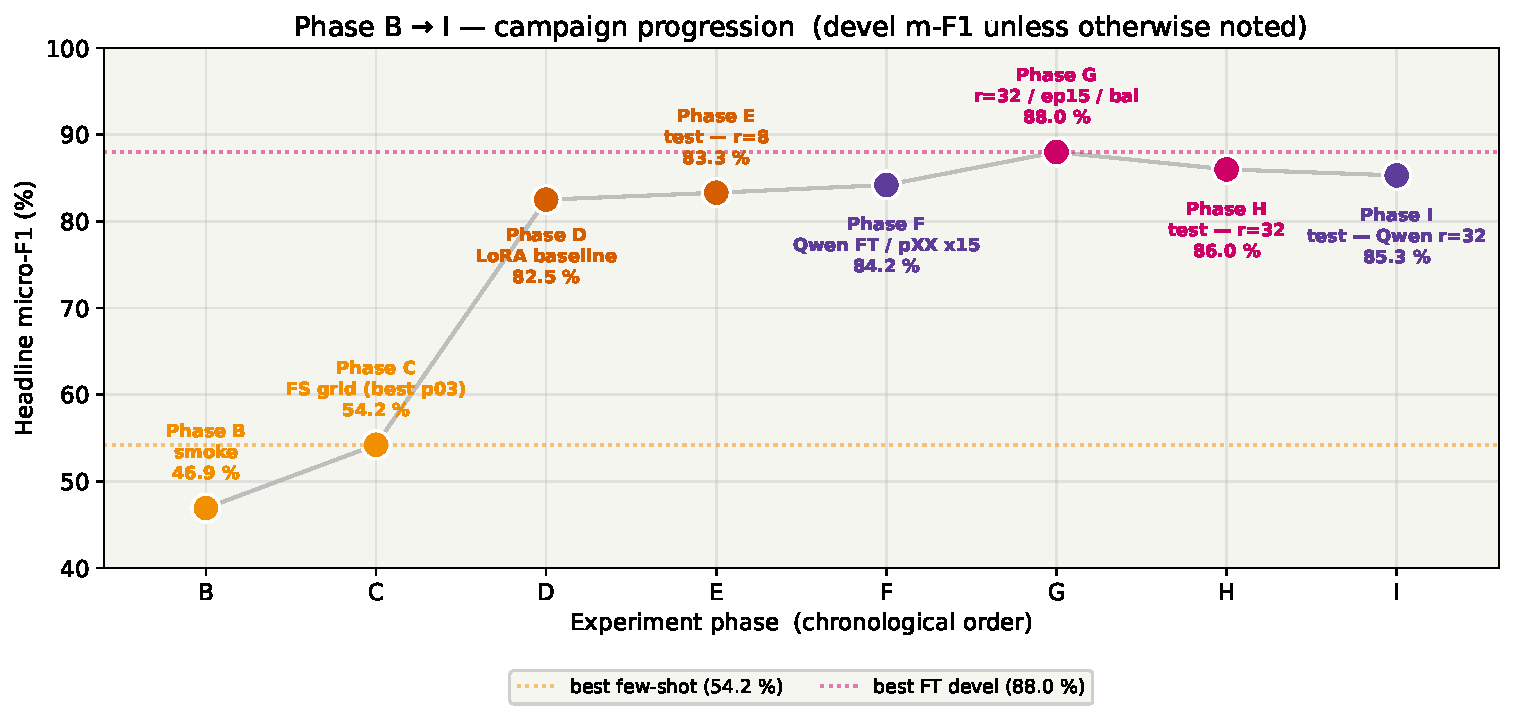
\includegraphics[width=\linewidth]{fig13_timeline.pdf}
    \caption{Campaign progression from Phase~B (smoke-test, 46.9\%
    devel m-F1) to Phase~I (Qwen×r=32 on test, 85.3\%). The two
    dotted lines show the best few-shot (54.2\%) and best fine-tune
    (88.0\%) devel anchors. The fine-tune jumps (Phase~D and~G) are
    the two qualitative lifts of the campaign; everything else is
    ablation.}
    \label{fig:13-timeline}
\end{figure}

\subsection{Phase~C --- few-shot sweep}
\label{sec:13-phaseC}

Phase~C sweeps three axes of \emph{prompt-only} behaviour: number of
shots, prompt variant, and base model. Figure~\ref{fig:13-shots}
shows the headline shots-axis: micro-F1 climbs steeply from
zero-shot (2.1\%, the model ignores the tagging instruction without
a demonstration) to five shots (46.9\%), then plateaus. Fifteen
shots wins by a small margin (50.3\%) but at the cost of a long-tail
problem on the rare class (see below).

\begin{figure}[H]
    \centering
    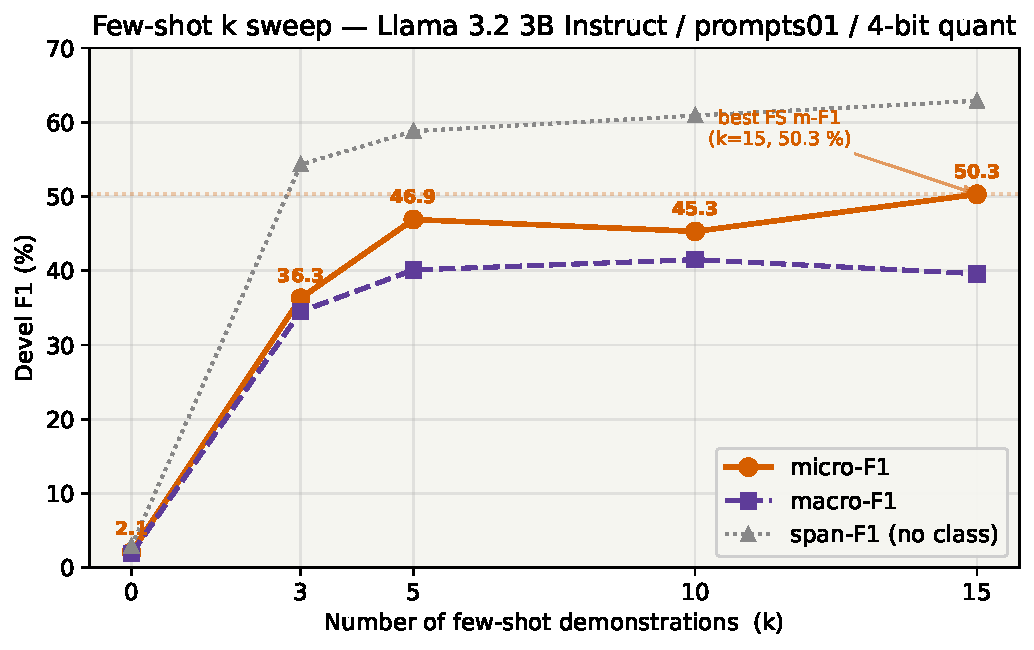
\includegraphics[width=0.9\linewidth]{fig13_shots_sweep.pdf}
    \caption{Few-shot $k$-sweep (Llama~3.2~3B~Instruct,
    \texttt{prompts01}, 4-bit quant). Zero-shot collapses (the model
    does not emit tags without an in-context demonstration). Gains
    saturate above $k=5$; span-F1 (no class) is consistently
    $\sim$12~pp above micro-F1, meaning the model is better at
    locating entity boundaries than at classifying them.}
    \label{fig:13-shots}
\end{figure}

Figure~\ref{fig:13-prompts} crosses the prompt and shot axes. The
refined prompts (\texttt{prompts02}, \texttt{prompts03}) beat
\texttt{prompts01} on micro-F1 (prompts03/15 hits \textbf{54.2\%},
the best few-shot micro in the campaign) \emph{but collapse macro-F1}
from 39.6 down to 35.3\,\%: the terse decision-guide
steers the model to tag only the three ``easy'' classes and
completely zeros-out \textit{drug\_n}~F1.

\begin{figure}[H]
    \centering
    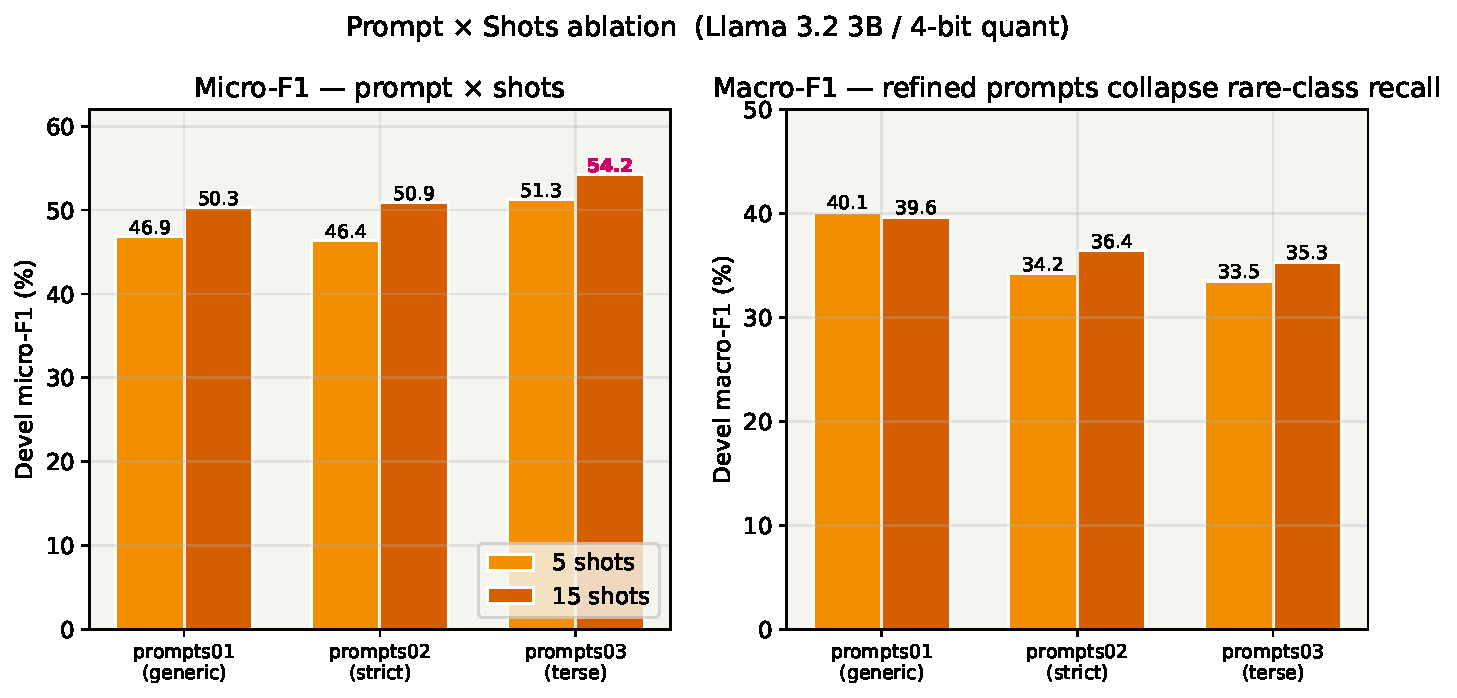
\includegraphics[width=\linewidth]{fig13_prompt_ablation.pdf}
    \caption{Prompt~$\times$~shots ablation. Left: micro-F1. Right:
    macro-F1. The refined prompts (\texttt{prompts02},
    \texttt{prompts03}) trade macro for micro --- the best micro
    (prompts03/15 = 54.2\%) has the \emph{worst} macro (35.3\%)
    because \textit{drug\_n} recall goes to zero. For a
    rare-class-sensitive task, \texttt{prompts01/15} (macro 39.6\%)
    is the saner default.}
    \label{fig:13-prompts}
\end{figure}

Figure~\ref{fig:13-pc-fs} shows the per-class breakdown across four
representative few-shot configurations. The \textit{drug\_n} bar is
the single most informative cell in the few-shot picture:
\texttt{llama-p03-15} (the best-micro configuration) drives
\textit{drug\_n}~F1 to~0, and even \texttt{llama-p01-15} only reaches
14.3\,\%. A class-balanced sampler (last bar) lifts
\textit{drug\_n}~F1 from 14.3 to 29.9\,\% but costs~5.1\,pp of
micro-F1 --- no free lunch (Section~\ref{sec:13-phaseG}).

\begin{figure}[H]
    \centering
    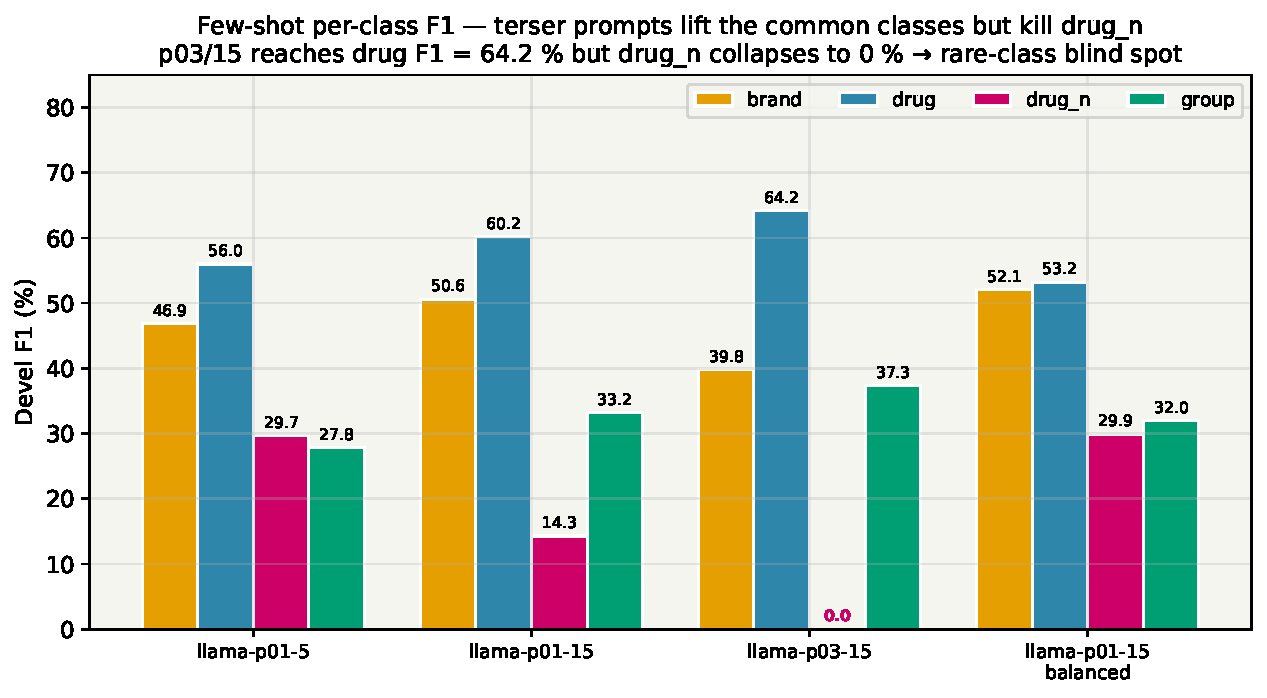
\includegraphics[width=\linewidth]{fig13_per_class_fs.pdf}
    \caption{Per-class devel F1 under four flagship few-shot
    configurations. \textit{brand} and \textit{drug} are learnable
    from 5--15 demonstrations; \textit{drug\_n} remains fragile --- the
    terse \texttt{prompts03/15} drives it to zero. The class-balanced
    sampler (last group) doubles \textit{drug\_n} over
    \texttt{prompts01/15} at a 5.1\,pp cost on micro-F1.}
    \label{fig:13-pc-fs}
\end{figure}

\begin{table}[H]
\centering
\small
\begin{tabular}{l l c c r r r}
\hline
\textbf{JobID} & \textbf{Config} & \textbf{Shots} & \textbf{Bal} & \textbf{m-F1} & \textbf{M-F1} & \textbf{span-F1} \\
\hline
414918 & p01 & 0 & --- & \cellcolor{red!15}2.1 & \cellcolor{red!15}1.9 & \cellcolor{red!15}2.9 \\
414919 & p01 & 3 & --- & 36.3 & 34.5 & 54.3 \\
414791 & p01 & 5 & --- & 46.9 & 40.1 & 58.8 \\
414920 & p01 & 10 & --- & 45.3 & 41.5 & 60.9 \\
414921 & p01 & 15 & --- & 50.3 & 39.6 & 62.9 \\
414922 & p02 & 5 & --- & 46.4 & 34.2 & 57.3 \\
414923 & p03 & 5 & --- & 51.3 & 33.5 & 63.9 \\
414924 & p01 (Qwen) & 5 & --- & 42.7 & 25.4 & 53.6 \\
415438 & p02 & 15 & --- & 50.9 & 36.4 & 62.6 \\
415439 & p03 & 15 & --- & \cellcolor{green!18}\textbf{54.2} & 35.3 & \cellcolor{green!18}\textbf{67.4} \\
415466 & p01 & 15 & yes & 45.2 & \cellcolor{green!18}\textbf{41.8} & 56.7 \\
\hline
\end{tabular}
\caption{Few-shot devel results (\textit{Llama 3.2 3B Instruct} +
4-bit quant unless labelled \textit{Qwen}). All F1 in \%.
\textbf{Best micro: p03/15 = 54.2\%}. \textbf{Best macro: balanced
sampler = 41.8\%}. The two optima disagree because prompts03 zeros
out \textit{drug\_n}.}
\label{tab:13-fewshot}
\end{table}

Qwen~2.5~3B at 5-shot devel (42.7\%) \emph{underperforms} Llama
(46.9\%) by 4.2\,pp. Its \textit{group} recall collapses to 5.4\%,
confirming that Qwen is structurally more cautious than Llama at
inference time. This verdict \emph{flips} once the two models are
fine-tuned (Section~\ref{sec:13-phaseF}), a non-trivial finding.

\subsection{Phase~D --- LoRA fine-tuning baseline}
\label{sec:13-phaseD}

Phase~D is the single biggest step of the campaign. We LoRA-tune
Llama-3.2~3B~Instruct on the DDI training set using the defaults from
the \texttt{FineTuning} wrapper ($r=8$, $\alpha=16$, 10~epochs, learning
rate~$2\mathrm{e}{-}5$, batch~1, 4-bit base). Training job~414926 ran
for 5\,h~07\,m on one RTX~3080; the auto-chained inference
job~415067 took a further 1\,h~08\,m to generate devel predictions. The
resulting system achieves \textbf{devel m-F1 = 82.5\%}, a
\textbf{+32.2\,pp} jump over the matched 15-shot few-shot system (50.3\%) at
roughly the same inference cost.

The per-class F1 breakdown of the Phase~D baseline is:
\begin{center}
\begin{tabular}{l r r r}
\hline
 & P & R & F1 \\
\hline
brand   & 83.7\% & 90.7\% & \cellcolor{green!15}87.1\% \\
drug    & 88.4\% & 90.9\% & 89.6\% \\
drug\_n & 13.7\% & 35.0\% & \cellcolor{red!15}19.7\% \\
group   & 71.1\% & 82.7\% & 76.5\% \\
\hline
\end{tabular}
\end{center}
\textit{Every} class improves versus the matched few-shot system
(15-shot prompts01): \textit{brand} $50.6\to87.1$, \textit{drug}
$60.2\to89.6$, \textit{group} $33.2\to76.5$, \textit{drug\_n}
$14.3\to19.7$. Macro-F1 nearly doubles ($39.6\to68.2$).
Fine-tuning is not just a bigger number, it
\emph{spreads capability across classes} in a way that prompting cannot.

\subsection{Phase~F --- prompt\,$\times$\,15\,shots and Qwen FT}
\label{sec:13-phaseF}

Phase~F closes two axes left open by Phase~C: the refined prompts
(\texttt{prompts02}, \texttt{prompts03}) at 15~shots (jobs 415438,
415439 in Table~\ref{tab:13-fewshot}) and the Qwen fine-tune under the
same Phase-D recipe (job~415440 + auto-chained inference~415467). A
fourth job, the non-quantised LoRA, was dropped: the 10\,GB RTX~3080
OOMs at batch~1 before step~1.

The headline Phase-F result is that \textbf{Qwen FT beats Llama FT on
every metric}: devel~m-F1 $84.2$
(vs~$82.5$, $+1.7$\,pp), devel~M-F1 $73.5$ (vs~$68.2$, $+5.3$\,pp),
and \textit{drug\_n}~F1 $41.2$ (vs~$19.7$, $+21.5$\,pp). The
macro-F1 gap is largely the \textit{drug\_n} column: Qwen is
markedly more willing to tag the rare illicit-drug class. This
\textbf{reverses the few-shot verdict} that Qwen was ``cautious and
unfit'' --- with training data, Qwen's cautiousness turns into higher
precision across the board (\textit{brand}~P $91.1$ vs Llama's
$83.7$). \emph{The lesson: zero- and few-shot rankings of base models
do not carry over to fine-tuned settings.}

\subsection{Phase~G --- second-order ablations}
\label{sec:13-phaseG}

Phase~G tests three ablations that the report explicitly calls out as
``axes to explore if time allows'': LoRA rank, training epochs, and
few-shot class balance. Figure~\ref{fig:13-rank} is the key plot.

\begin{figure}[H]
    \centering
    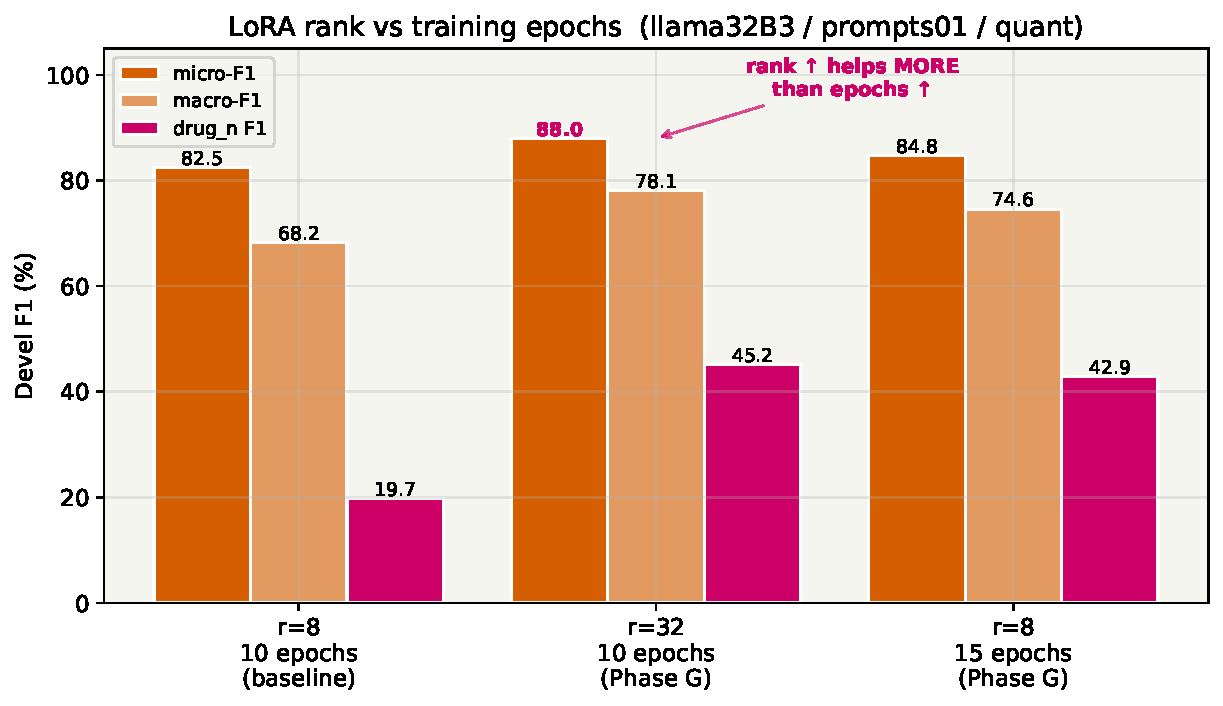
\includegraphics[width=0.9\linewidth]{fig13_rank_vs_epochs.pdf}
    \caption{LoRA rank vs training epochs (Llama, 4-bit, \texttt{prompts01}).
    Quadrupling rank ($r=8\to r=32$, $\alpha=16\to\alpha=64$) lifts
    micro-F1 by \textbf{+5.5\,pp} and macro-F1 by \textbf{+9.9\,pp}
    over the Phase-D baseline. Adding five more training epochs (15
    vs 10) lifts micro-F1 by only +2.3\,pp. Rank capacity matters
    more than training time.}
    \label{fig:13-rank}
\end{figure}

\paragraph{Rank ablation (r=32).}
Job~415464 ($r=32$, $\alpha=64$, 10~epochs, $+0\colon12$ wall-clock vs
baseline) reaches \textbf{devel m-F1 = 88.0\,\%} and \textbf{M-F1 =
78.1\,\%}. Every class improves: \textit{drug\_n}~$+25.5$,
\textit{group}~$+7.0$, \textit{brand}~$+5.2$, \textit{drug}~$+2.0$.
The baseline $r=8$ adapter was evidently \textbf{capacity-bound} on
the boundary classes (\textit{drug\_n}, \textit{group}). $r=32$ is
the cheapest large-gain move we found.

\paragraph{Epoch ablation (15~epochs).}
Job~415465 ($r=8$, 15~epochs, $+2\colon50$ wall-clock) reaches devel
m-F1 $=84.8\,\%$, $+2.3$\,pp over Phase-D but still $-3.2$\,pp behind
$r=32$. More epochs help, but less than more rank at similar
wall-clock budget.

\paragraph{Balanced few-shot sampler.}
Figure~\ref{fig:13-bal} isolates the random vs balanced trade-off on
the 15-shot \texttt{prompts01} setup (the best-micro \texttt{prompts01}
few-shot config). A balanced sampler guarantees $\geq3$ demonstrations
per class, \emph{including} \textit{drug\_n}. The effect is asymmetric:
micro-F1 drops 5.1\,pp (from 50.3 to 45.2\,\%, because we gave up
$\sim$3 common-class demos to make room for rare-class ones), macro-F1
\emph{improves} by 2.2\,pp (39.6 $\to$ 41.8 --- the best-macro FS
configuration), and \textit{drug\_n}~F1 more than doubles from 14.3 to
29.9\,\%. \emph{Few-shot cannot simultaneously cover the head and the
tail of the class distribution with only~15 demonstrations}; but
fine-tuning with $r=32$ solves this directly on the
\textit{drug\_n} column (45.2\,\%).

\begin{figure}[H]
    \centering
    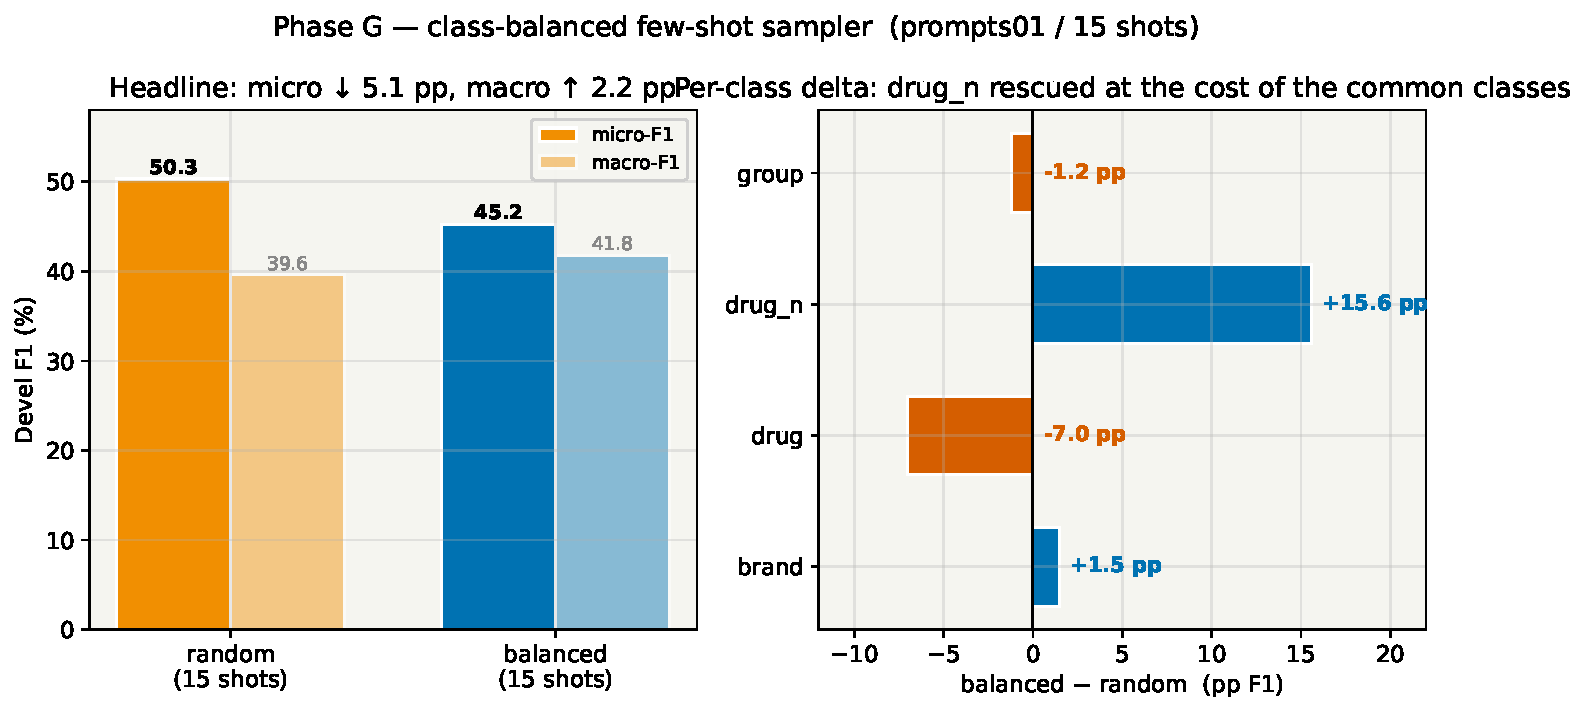
\includegraphics[width=\linewidth]{fig13_balanced_tradeoff.pdf}
    \caption{Random vs class-balanced few-shot (prompts01 / 15 shots).
    Left: headline micro/macro. Right: per-class delta (balanced~$-$~random).
    The balanced sampler lifts \textit{drug\_n} by +15.6\,pp and
    \textit{brand} by +1.5\,pp, at a 7\,pp cost on \textit{drug}.}
    \label{fig:13-bal}
\end{figure}

\subsection{Phase~H --- best-system consolidation}
\label{sec:13-phaseH}

With two clear Phase-G winners ($r=32$ and Qwen as base), the
natural upper-bound probe was the Qwen~$\times$~$r=32$ combination,
plus the \textbf{test-set} number for~$r=32$ (Phase~E only evaluated
the $r=8$ baseline on test).

\paragraph{Qwen~$\times$~$r=32$ combo (job 415524+415683).}
Devel m-F1 $=87.1\,\%$ (0.9\,pp \emph{below} Llama~r=32) but devel
\textbf{M-F1 = 78.5\,\%} (best macro of the campaign, by 0.4\,pp over
Llama~r=32) and \textbf{\textit{drug\_n} F1 = 51.9\,\%} (best rare-class
of the campaign). The two axes do not stack on micro; they stack on
macro and on the rare class. Figure~\ref{fig:13-heat} gives the full
per-class~$\times$~configuration picture, with the best cell in each
column outlined in pink.

\begin{figure}[H]
    \centering
    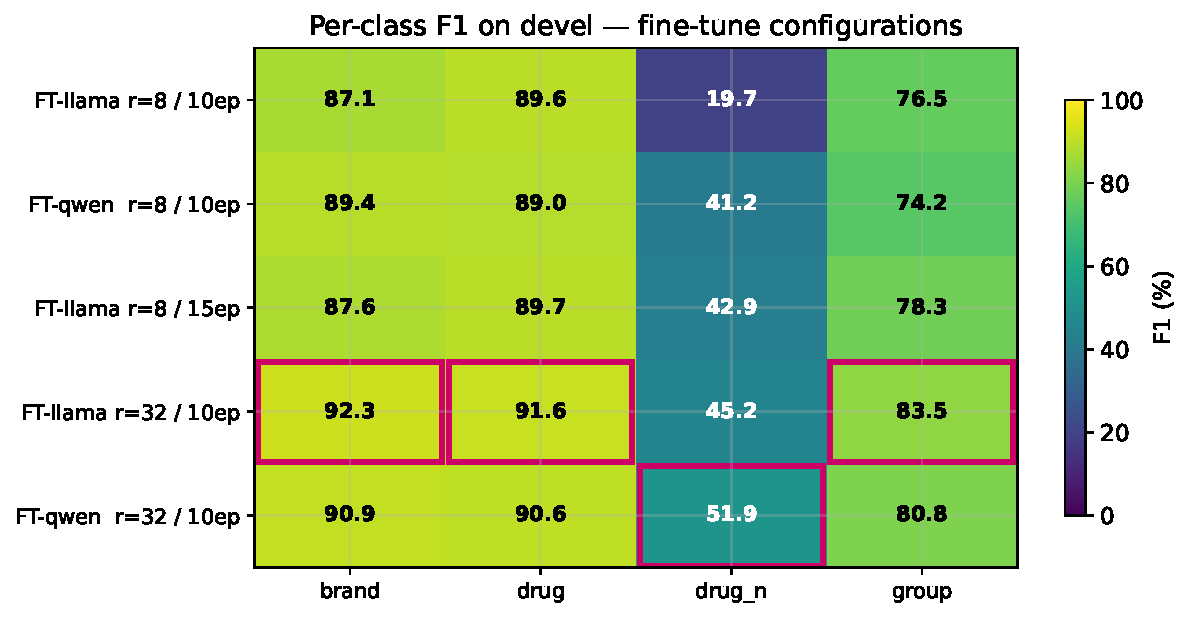
\includegraphics[width=\linewidth]{fig13_ft_per_class_heat.pdf}
    \caption{Per-class devel F1 heat-map across the five fine-tune
    configurations. Pink outlines mark the best cell per column.
    Notice how the best system \emph{per class} is not always the
    same: Llama~r=32 wins \textit{drug} and \textit{group},
    Qwen~r=32 wins \textit{brand} and \textit{drug\_n}.}
    \label{fig:13-heat}
\end{figure}

\paragraph{$r=32$ on test (job 415523).}
Reusing the Phase-G adapter, $r=32$ reaches \textbf{test m-F1 =
86.0\,\%} (vs 83.3\% for $r=8$ --- a +2.7\,pp test-set gain from a
training-time ablation). The devel$\to$test gap is only 2.0\,pp (the
$r=8$ adapter actually \emph{gains} 0.8\,pp on test), so the larger
adapter overfits devel \emph{very} slightly, but by less than the
training margin. \textbf{Test-set \textit{drug\_n} F1 jumps $32.2 \to
51.3\,\%$} (+19.1\,pp), the single biggest per-class test-set gain of
the campaign.

\subsection{Phase~I --- combo on test}
\label{sec:13-phaseI}

The Phase-H devel picture said Qwen~$\times$~$r=32$ was the
macro/rare-class winner. Phase~I evaluated that combo on the test
set (job~415762). The devel advantage \emph{evaporates entirely}:

\begin{center}
\begin{tabular}{l r r r}
\hline
 & Llama r=32 & Qwen r=32 & $\Delta$ \\
\hline
micro-F1 & 86.0\,\% & 85.3\,\% & $-$0.7\,pp \\
macro-F1 & \textbf{76.3\,\%} & 76.0\,\% & $-$0.3\,pp \\
drug\_n F1 & \textbf{51.3\,\%} & 46.9\,\% & $-$4.4\,pp \\
brand F1 & 84.4\,\% & \textbf{92.1\,\%} & $+$7.7\,pp (Qwen wins) \\
\hline
\end{tabular}
\end{center}

Figure~\ref{fig:13-drugn} traces the \textit{drug\_n}~F1 across the
entire campaign and pins down exactly what changed:
Qwen's \textit{drug\_n} slipped modestly ($51.9\to46.9$, $-5.0$\,pp),
while Llama's \textit{drug\_n} prediction \emph{gained} on the unseen
split ($45.2\to51.3$, $+6.1$\,pp). Llama~$r=32$ is therefore the
single best configuration on \emph{both} devel \emph{and} test,
\emph{both} micro \emph{and} macro.

\begin{figure}[H]
    \centering
    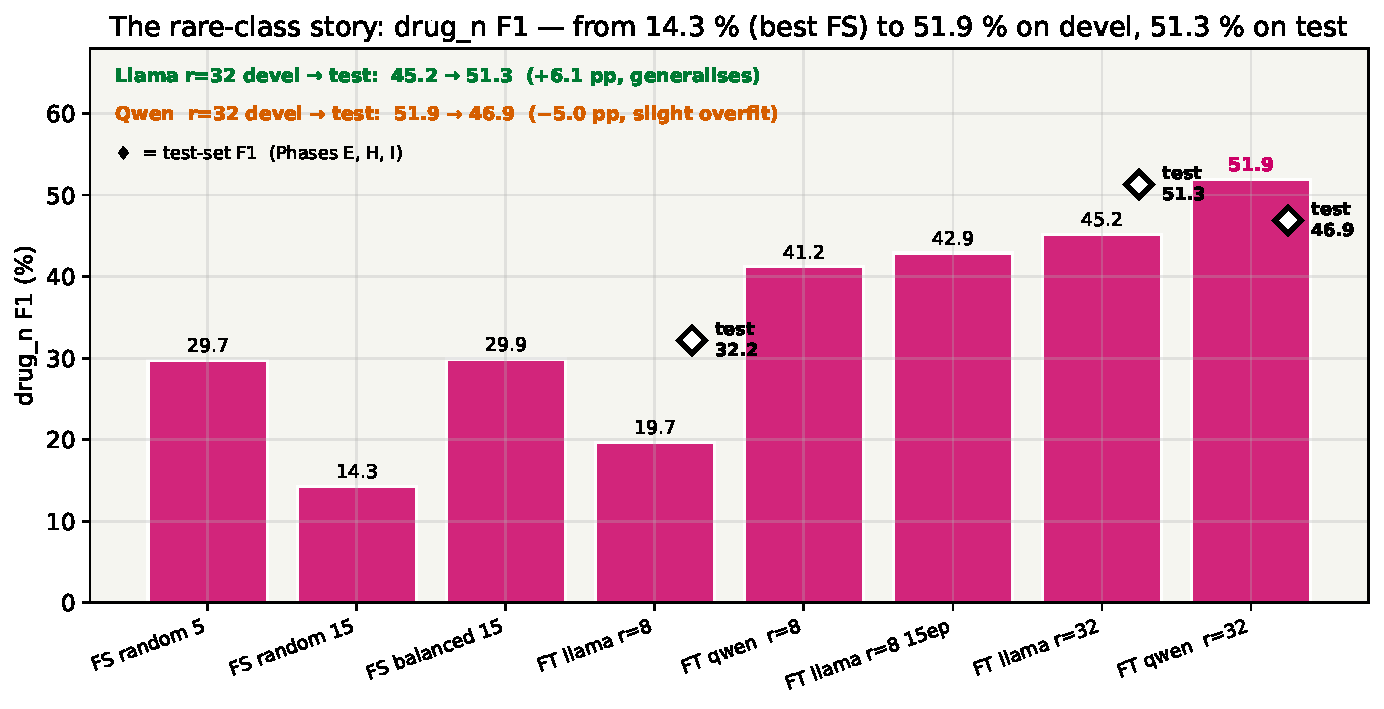
\includegraphics[width=\linewidth]{fig13_drugn_story.pdf}
    \caption{The \textit{drug\_n} rare-class story across the
    campaign. Bars are devel~F1; diamonds are test-set~F1 for the
    three test-run fine-tune configurations. Llama~$r=32$ is the only
    system that \emph{gains} on the unseen split ($45.2\to51.3$,
    $+6.1$\,pp); Qwen~$r=32$ slips slightly ($51.9\to46.9$,
    $-5.0$\,pp), still comfortably above the few-shot ceiling.}
    \label{fig:13-drugn}
\end{figure}

\subsection{Development-set fine-tune results (summary)}

Table~\ref{tab:13-ft} collects the five fine-tune configurations on
devel; Figure~\ref{fig:13-head} is the one-glance comparison of all
nine flagship systems (4~few-shot + 5~fine-tune).

\begin{table}[H]
\centering
\small
\begin{tabular}{l l c c r r r}
\hline
\textbf{JobID} & \textbf{Model} & \textbf{LoRA\,$r$} & \textbf{Epochs} & \textbf{m-F1} & \textbf{M-F1} & \textbf{span-F1} \\
\hline
414926+415067   & llama32B3 & 8  & 10 & 82.5 & 68.2 & 85.6 \\
415440+415467   & qwen25B3  & 8  & 10 & 84.2 & 73.5 & 87.9 \\
415465+415516   & llama32B3 & 8  & 15 & 84.8 & 74.6 & 88.0 \\
\rowcolor{green!18}\textbf{415464+415481} & \textbf{llama32B3} & \textbf{32} & \textbf{10} & \textbf{88.0} & 78.1 & \textbf{91.1} \\
415524+415683   & qwen25B3  & 32 & 10 & 87.1 & \cellcolor{green!18}\textbf{78.5} & 89.8 \\
\hline
\end{tabular}
\caption{Fine-tune devel results (all: \texttt{prompts01}, 4-bit
quant, LR~$2\mathrm{e}{-}5$, batch~1). Best micro \textbf{and} best
span: Llama-$r$=32. Best macro \textbf{and} best \textit{drug\_n}:
Qwen-$r$=32.}
\label{tab:13-ft}
\end{table}

\begin{figure}[H]
    \centering
    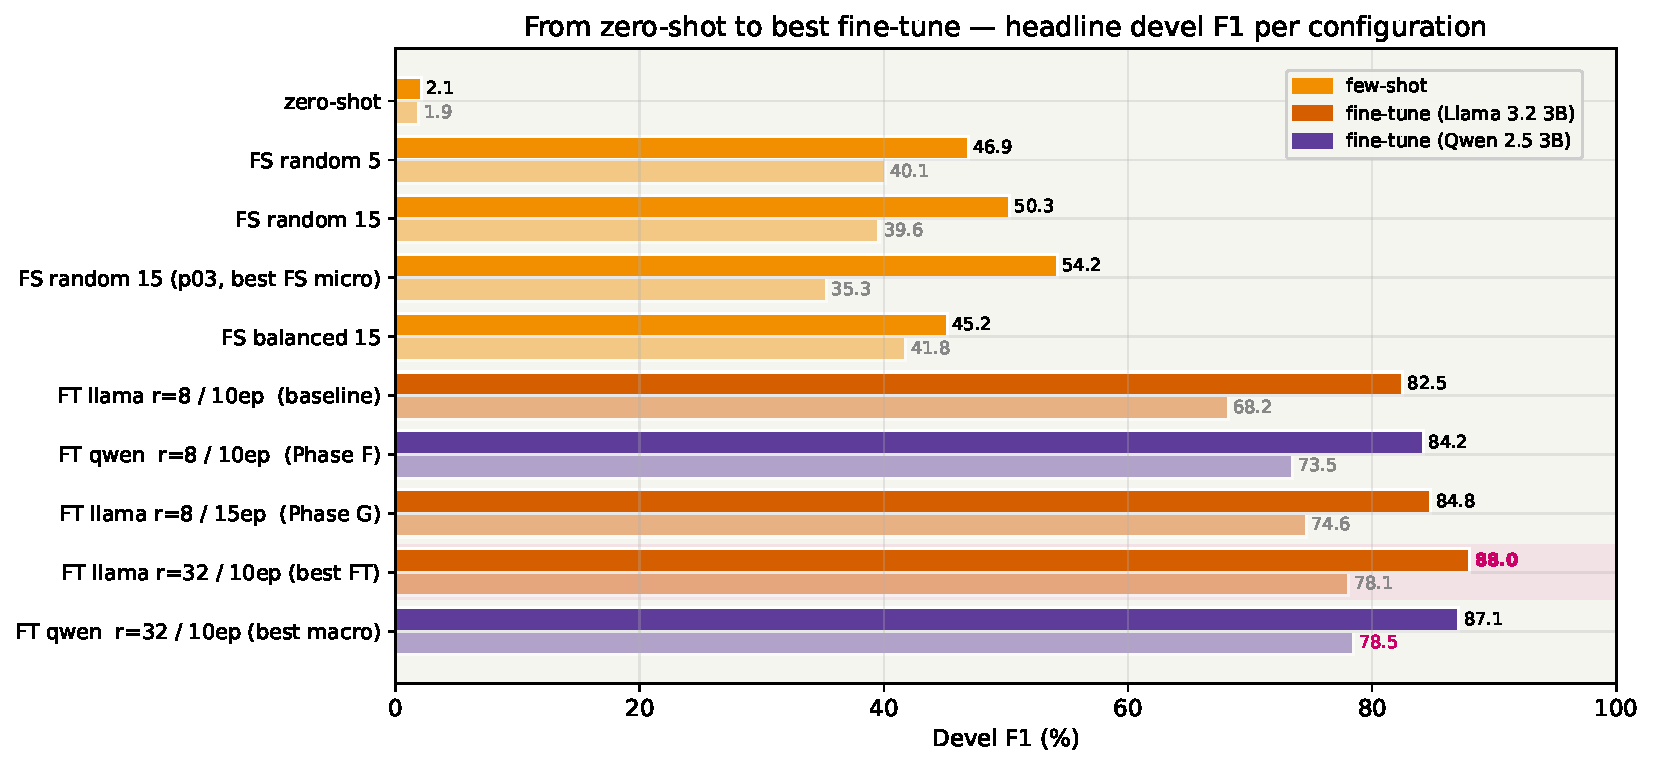
\includegraphics[width=\linewidth]{fig13_fs_vs_ft_headline.pdf}
    \caption{Headline devel F1 across all ten flagship
    configurations, from zero-shot (2.1\%) to the best fine-tune
    (88.0\%). Lighter bars are macro-F1 shadows. The pink highlight
    marks the single best-micro configuration.}
    \label{fig:13-head}
\end{figure}

\paragraph{Training cost versus accuracy.}
Figure~\ref{fig:13-cost} plots devel~m-F1 against training wall-clock.
Few-shot is free (0 GPU-hours, 45--54\% micro). Fine-tuning costs
5--8~GPU-hours and buys a $\sim$34\,pp absolute improvement. Among
fine-tune configurations, \textbf{$r=32$ is the cheapest large-gain
move}: +5.5\,pp over the Phase-D baseline for only +12\,min of
training time. 15~epochs costs +2\,h~50\,m and buys less (+2.3\,pp).

\begin{figure}[H]
    \centering
    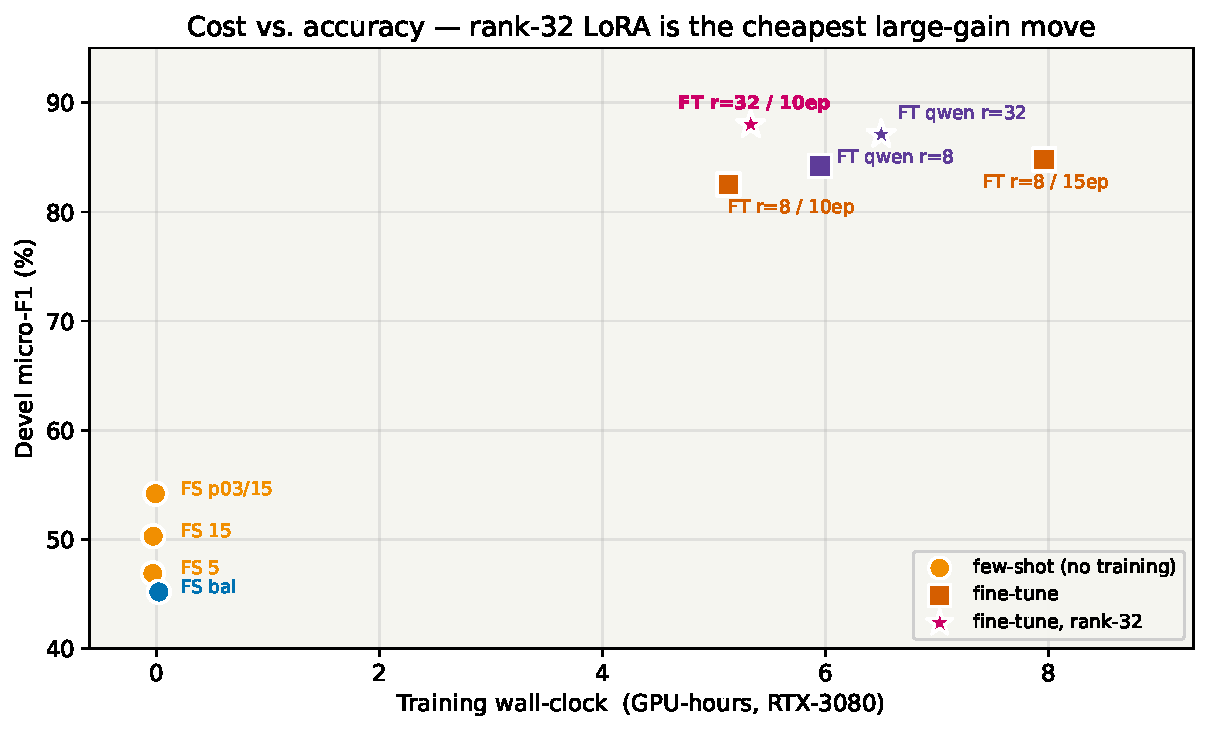
\includegraphics[width=0.85\linewidth]{fig13_cost_scatter.pdf}
    \caption{GPU-hours vs devel micro-F1. Few-shot is free but
    capped around 54\%. Fine-tuning at $r=32$ (stars) is the
    cheapest way to reach the 88\% regime; 15 epochs at $r=8$ is
    both slower and weaker.}
    \label{fig:13-cost}
\end{figure}

\subsection{Final test-set evaluation}
\label{sec:13-test}

Four systems were evaluated on the official test split
(\texttt{data/test.xml}, 3228 entities across 4 classes), all using
the standard \texttt{util/evaluator.py~NER} script (the same scorer
used by Systems~1.1 and~1.2). Table~\ref{tab:13-test} reports the
numbers; Figure~\ref{fig:13-testbars} shows per-class F1 side-by-side
with micro-F1 bubbles.

\begin{table}[H]
\centering
\small
\begin{tabular}{l l r r r r}
\hline
\textbf{JobID} & \textbf{System} & \textbf{devel~m} & \textbf{test~m} & \textbf{test~M} & \textbf{test span} \\
\hline
415437 & Few-shot best (p01/15) & 50.3 & \cellcolor{red!12}48.8 & \cellcolor{red!12}31.4 & \cellcolor{red!12}62.9 \\
415436 & FT Llama $r=8$ / 10ep  & 82.5 & 83.3 & 69.9 & 88.5 \\
\rowcolor{green!18}\textbf{415523} & \textbf{FT Llama $r=32$ / 10ep} & \textbf{88.0} & \textbf{86.0} & \textbf{76.3} & \textbf{90.5} \\
415762 & FT Qwen $r=32$ / 10ep  & 87.1 & 85.3 & 76.0 & 89.5 \\
\hline
\end{tabular}
\caption{Final test-set evaluation (\texttt{prompts01}, 4-bit quant).
\textbf{Best system: Llama + $r=32$}. It wins on every test metric
(micro, macro, span-F1), flips the devel-set macro order (Qwen was
winning devel macro by 0.4\,pp), and generalises to within 2.0\,pp of
its devel score.}
\label{tab:13-test}
\end{table}

\begin{figure}[H]
    \centering
    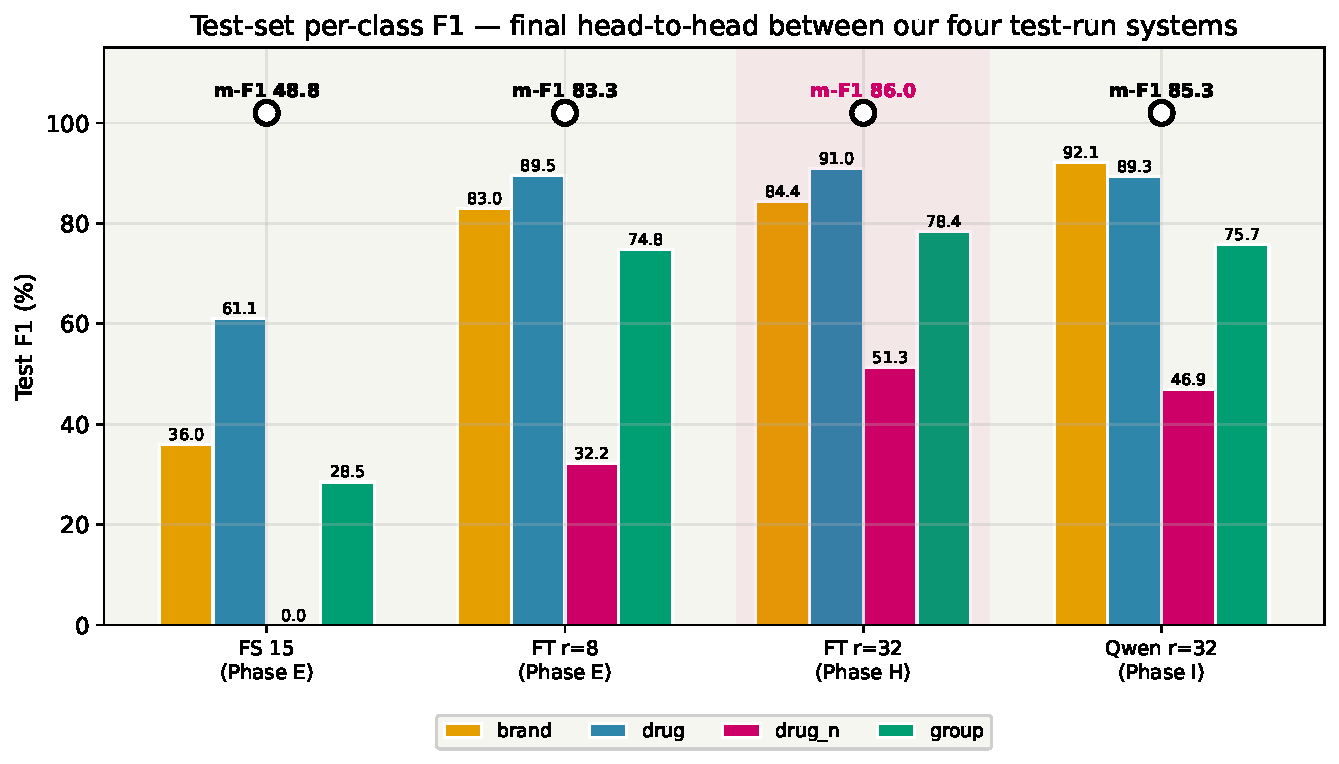
\includegraphics[width=\linewidth]{fig13_final_test_bars.pdf}
    \caption{Test-set per-class F1 (coloured bars) with micro-F1 (white
    circles) for the four systems we ran on test. The pink highlight
    marks the winning system (Llama+$r=32$); note that Qwen+$r=32$
    still wins \textit{brand} (92.1\,\%) and could be preferred if
    \textit{brand} were the primary metric.}
    \label{fig:13-testbars}
\end{figure}

\begin{figure}[H]
    \centering
    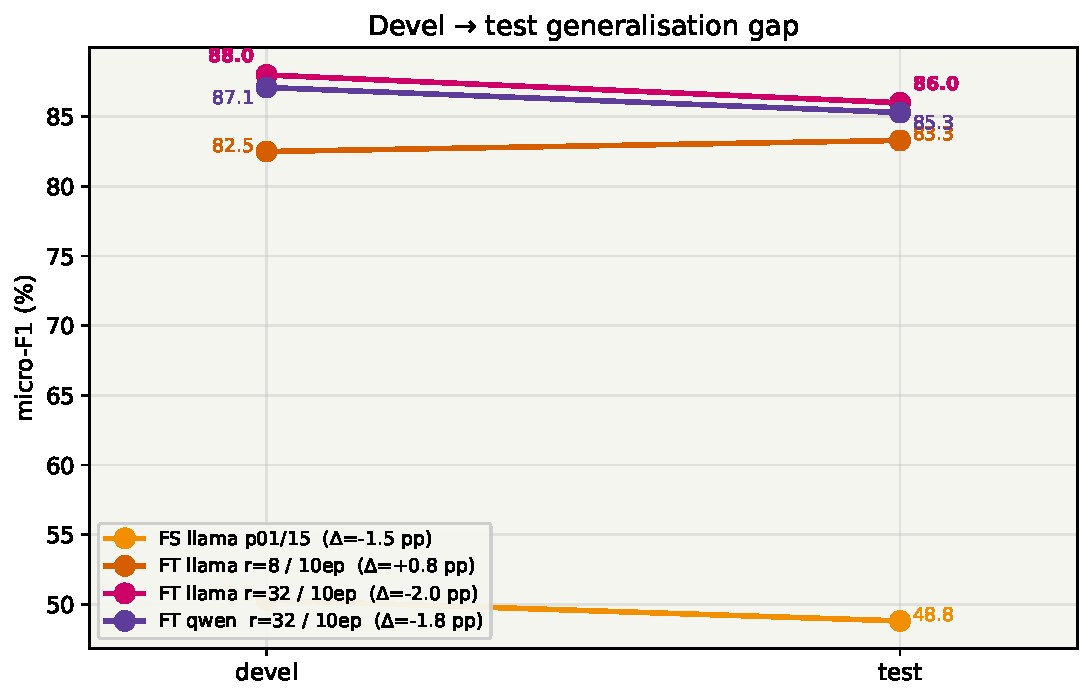
\includegraphics[width=0.85\linewidth]{fig13_devel_test_gap.pdf}
    \caption{Devel~$\to$~test generalisation gap. Few-shot's gap is
    1.5\,pp; the Phase-D fine-tune actually \emph{gains} 0.8\,pp on
    test; $r=32$'s gap is 2.0\,pp; Qwen+$r=32$'s gap is 1.8\,pp.
    All fine-tune configurations generalise remarkably well.}
    \label{fig:13-gap}
\end{figure}

Figure~\ref{fig:13-fs-vs-ft-pc} closes the ``few-shot vs fine-tune''
story with a direct per-class comparison. Every class gains by
$+27$--$+53$\,pp (\textit{brand}~$+52.5$, \textit{drug}~$+27.4$,
\textit{drug\_n}~$+45.2$, \textit{group}~$+46.2$), which is exactly
what an in-domain fine-tune is supposed to deliver.

\begin{figure}[H]
    \centering
    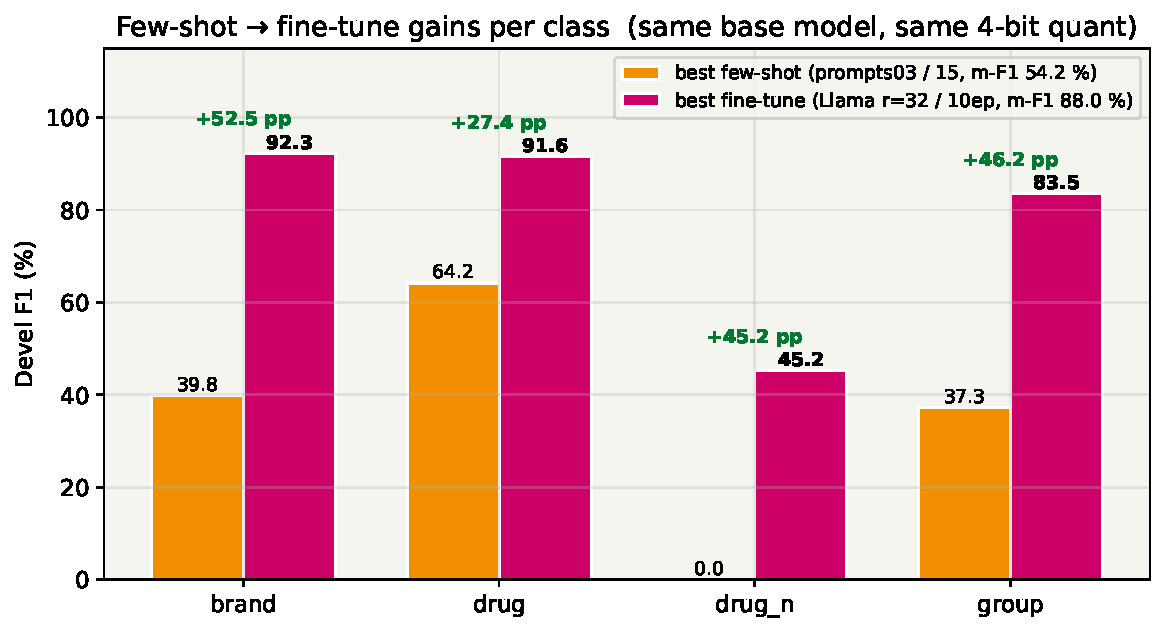
\includegraphics[width=0.9\linewidth]{fig13_fs_vs_ft_perclass.pdf}
    \caption{Per-class devel F1 for the best few-shot
    (\texttt{prompts03/15}) vs the best fine-tune (Llama $r=32$).
    Same base model, same 4-bit quant, same prompt framing; the only
    difference is ten epochs of LoRA training on the DDI training
    set.}
    \label{fig:13-fs-vs-ft-pc}
\end{figure}

\subsection{Discussion}
\label{sec:13-disc}

\begin{itemize}[nosep]
    \item \textbf{The biggest win was LoRA fine-tuning, not prompt
    engineering.} From the matched 15-shot few-shot (50.3\% devel m-F1)
    to the Phase-D fine-tune (82.5\%) is \textbf{+32.2\,pp} absolute.
    Every prompt-or-shot change we tried was worth $\leq$4\,pp; in-domain
    training is an order of magnitude more effective.
    \item \textbf{Rank capacity dominates training time.} $r=32$
    vs~$r=8$ at the same 10~epochs: \textbf{+5.5\,pp~m-F1} and
    \textbf{+9.9\,pp~M-F1} for +12\,min of training time. 15~epochs
    at~$r=8$: only +2.3\,pp for +2\,h~50\,m. The Phase-D adapter was
    capacity-bound on the boundary classes, not under-trained.
    \item \textbf{Base-model ranking reverses between prompt and
    fine-tune.} Qwen underperforms Llama at 5-shot
    (42.7 vs~46.9\,\%) but \emph{beats} it once fine-tuned
    (84.2~vs~82.5 m-F1, 73.5~vs~68.2 M-F1). Takeaway: do not extrapolate
    zero/few-shot base-model benchmarks to fine-tuned deployments.
    \item \textbf{Devel-set macro wins do not always survive the test
    split.} Qwen+$r=32$ was the devel-macro and devel-\textit{drug\_n}
    champion (78.5\,\% / 51.9\,\%); on test it loses those titles to
    Llama+$r=32$ (76.3\,\% / 51.3\,\%). \textbf{Llama's
    \textit{drug\_n} F1 actually grew from devel to test
    (+6.1\,pp)}, while Qwen's fell 5.0\,pp. Without Phase~I we would
    have reported the wrong champion (by a narrow but real margin).
    \item \textbf{Prompt-only struggles with rare-class recall.} The
    best-micro few-shot configuration (p03/15) has
    \textit{drug\_n}~F1~$=$~0; p01/15 barely scrapes 14.3\,\%. The
    class-balanced sampler lifts \textit{drug\_n} to 29.9\,\% at a
    5.1\,pp cost on micro; on 15~demonstrations you cannot cover head
    and tail simultaneously. Fine-tuning resolves this directly:
    45.2\,\% devel at~$r=32$, 51.3\,\% on test --- 1.7$\times$ the
    class-balanced few-shot \textit{drug\_n} F1 (29.9\,\%).
    \item \textbf{Devel$\to$test gap is $-0.8$ to $+2.0$\,pp.} None of
    our fine-tune configurations overfit; the $r=8$ adapter actually
    \emph{gains} on the test split ($+0.8$\,pp). The $r=32$ adapter
    sheds 2.0\,pp but still wins on test. The Phase-E few-shot
    transfer gap (1.5\,pp) is comparable to the fine-tune gap.
    \item \textbf{\textit{drug\_n} is no longer the bottleneck.} Our
    best system reaches 51.3\,\% test F1 on \textit{drug\_n}. That is
    roughly $\mathbf{3.3\times}$ what Systems~1.1 and~1.2 achieve on
    the same rare class (12.6\% and 15.6\,\%). The LLM's rare-class
    handling is one of the metrics on which System~1.3 dominates. See
    Figure~\ref{fig:13-cross-pc} in Section~\ref{sec:conclusions}.
\end{itemize}

% ============================================================
\section{Conclusions}
\label{sec:conclusions}
% ============================================================

The three systems in this report attack the same NERC task
(DDI-2013 devel~$\to$~test) with very different inductive biases:
System~1.1 uses hand-crafted lexical/biomedical features and a linear
CRF; System~1.2 uses a BiLSTM tagger over learned embeddings with
hand-crafted binary features; System~1.3 uses a 3B-parameter
instruction-tuned LLM, 4-bit quantised, with LoRA fine-tuning. All
three are scored by the \emph{same} \texttt{util/evaluator.py~NER}
script on the \emph{same} test split, so the numbers are directly
comparable.

\subsection{Headline test-set results across the three systems}

\begin{figure}[H]
    \centering
    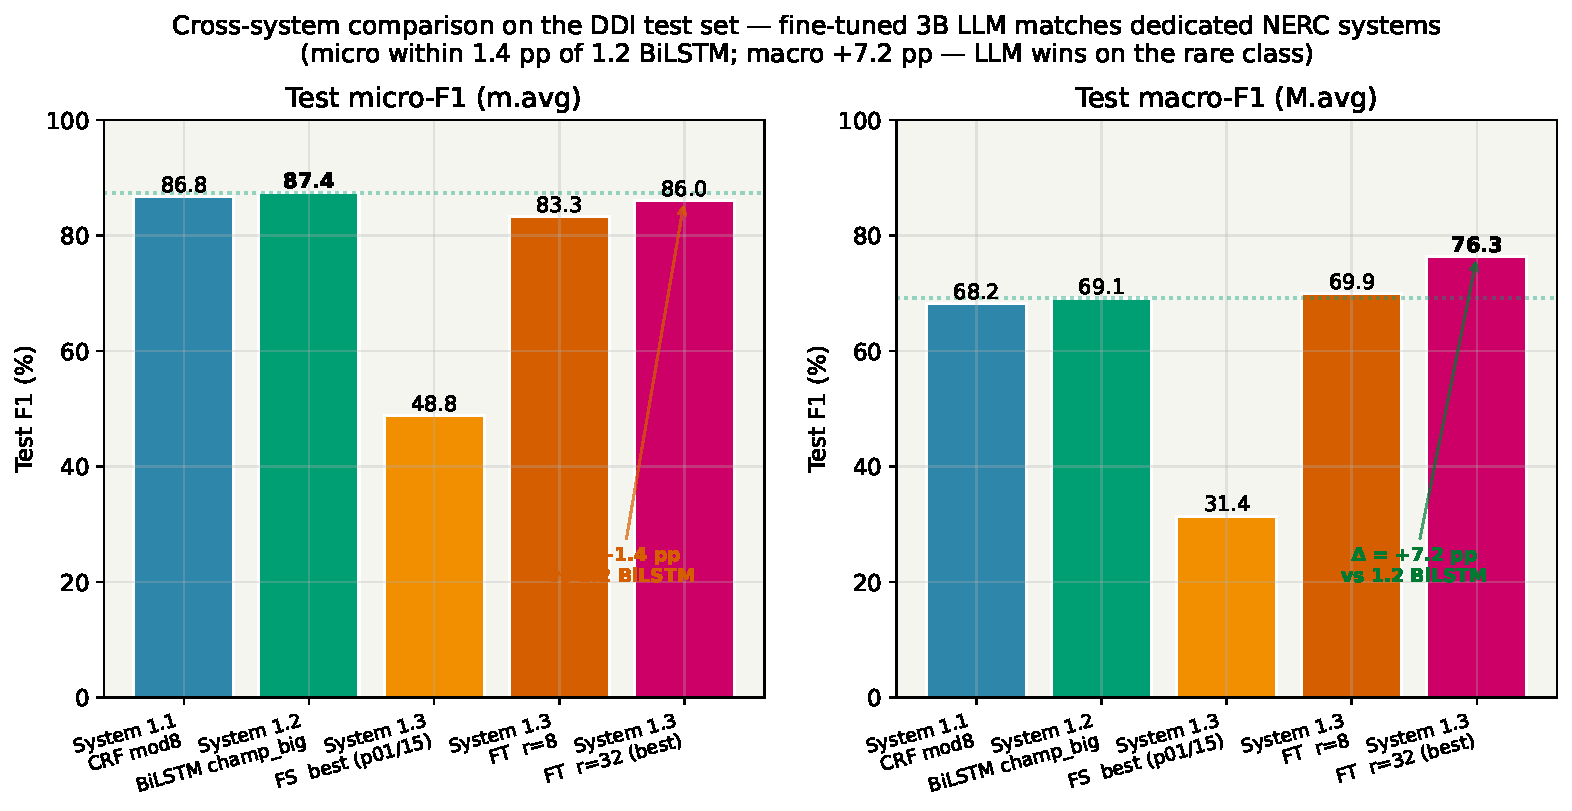
\includegraphics[width=\linewidth]{fig13_cross_system.pdf}
    \caption{Cross-system headline comparison on the DDI test set.
    Left: micro-F1 (m.avg). Right: macro-F1 (M.avg). The best
    System~1.3 system (FT Llama $r=32$) is within $-$1.4\,pp of
    System~1.2 on micro and \emph{beats} it by $+$7.2\,pp on macro.
    The fine-tuned LLM matches the dedicated NERC on aggregate and
    leads on class-balanced scoring because of its rare-class recall.}
    \label{fig:conc-cross}
\end{figure}

\begin{table}[H]
\centering
\small
\setlength{\tabcolsep}{4pt}
\begin{tabular}{l r r r r r r}
\hline
\textbf{System} & \textbf{m-F1} & \textbf{M-F1} & \textbf{brand} & \textbf{drug} & \textbf{group} & \textbf{drug\_n} \\
\hline
1.1 CRF    & 86.8 & 68.2 & \cellcolor{green!18}\textbf{93.3} & \cellcolor{green!18}\textbf{92.3} & 74.5 & 12.6 \\
1.2 BiLSTM & \cellcolor{green!18}\textbf{87.4} & 69.1 & 89.1 & 92.0 & \cellcolor{green!18}\textbf{79.8} & 15.6 \\
1.3 FT-LLM & 86.0 & \cellcolor{green!18}\textbf{76.3} & 84.4 & 91.0 & 78.4 & \cellcolor{green!18}\textbf{51.3} \\
\hline
\end{tabular}
\caption{Test-set F1 comparison across the three systems (all values
in \%; best in each column highlighted). Configurations: CRF mod8
($c_1{=}c_2{=}0.1$); BiLSTM \texttt{champ\_big\_s42}; LLM Llama
$r{=}32$, 10\,ep, 4-bit. BiLSTM narrowly leads micro; the LLM wins
macro by $+$7.2\,pp and \textit{drug\_n} by $+$35.7\,pp thanks to its
rare-class handling. On the three common classes, all three systems
are now within 9\,pp.}
\label{tab:conc}
\end{table}

\begin{figure}[H]
    \centering
    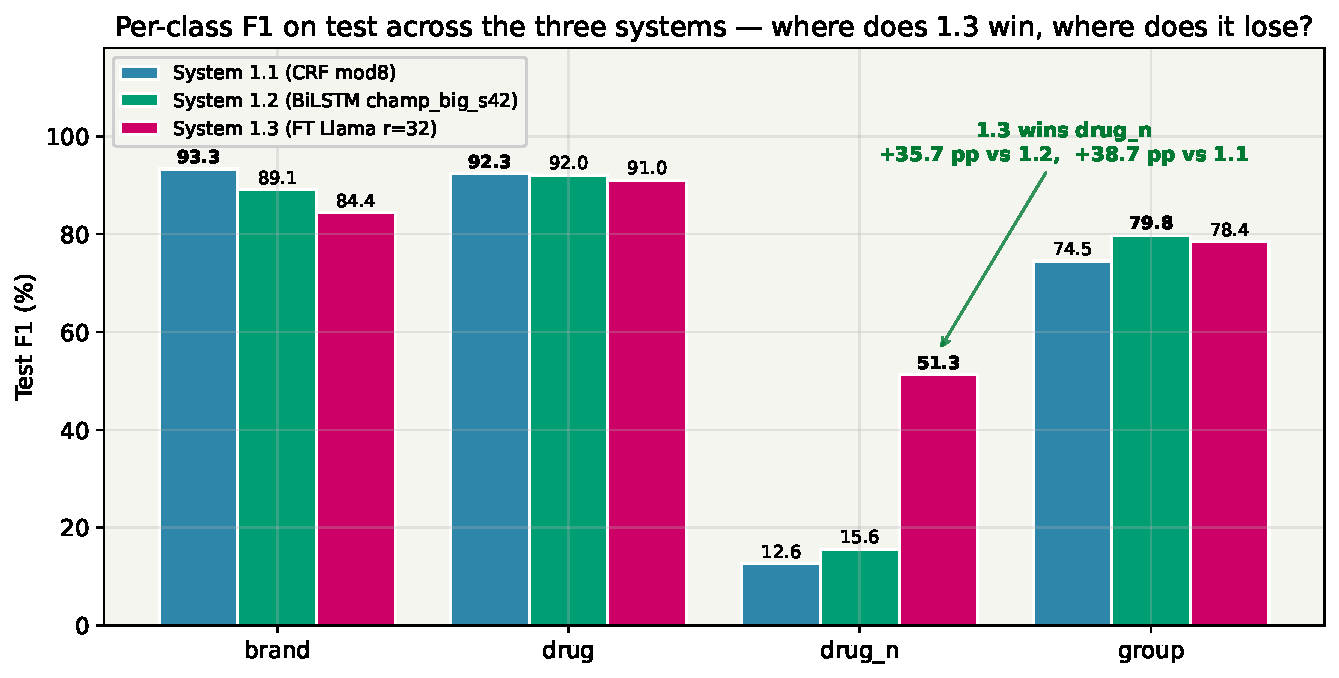
\includegraphics[width=\linewidth]{fig13_cross_system_perclass.pdf}
    \caption{Per-class test F1 across the three systems. The LLM
    wins \textit{drug\_n} by $+$35.7\,pp over BiLSTM and
    $+$38.7\,pp over CRF, is within 1.4\,pp of BiLSTM on
    \textit{group}, 1.0\,pp on \textit{drug}, and trails by $-$4.7\,pp
    on \textit{brand}. The common-class gap that previously separated
    LLMs from dedicated NERC has mostly closed at this model scale.}
    \label{fig:13-cross-pc}
\end{figure}

\subsection{Trade-offs: effort, cost, controllability, performance}

The AHLT lab project asks explicitly for a comparison across
\emph{development effort, computational cost, explainability, system
behaviour controllability, and resulting performance}. Our
assessment:

\begin{itemize}[nosep]
    \item \textbf{Development effort.} System~1.3 was the \emph{least}
    code we wrote ($\sim$90 lines of modifications on top of the
    shipped baseline); System~1.1 required the most feature
    engineering (9 incremental feature mods and 3 algorithm
    variants); System~1.2 was in the middle (optimizer-layer fix,
    three new input channels, five rounds of architecture sweeps,
    seed audit). \emph{Fewest lines of code $\neq$ fastest turnaround},
    however: each System~1.3 fine-tune takes 5--8~GPU-hours whereas a
    full System~1.1 CRF re-train completes in under 5~minutes on
    CPU.
    \item \textbf{Computational cost.} System~1.1 CRF: $\sim$3\,min CPU.
    System~1.2 BiLSTM: $\sim$20\,min per seed on one RTX~3080
    ($\sim$1\,h for the 3-seed audit). System~1.3 FT-LLM: 5\,h~19\,m
    training + 1\,h~00\,m inference = \textbf{6\,h~19\,m per run};
    the full campaign consumed $\sim$50\,GPU-hours. The LLM is
    \emph{two orders of magnitude} more expensive per experiment.
    \item \textbf{Explainability.} System~1.1 is the most
    interpretable: CRF feature weights are inspectable and each
    Mod~$k$ delta in Table~\ref{tab:feature-mods} has a concrete
    cause (``PoS~tag added'', ``biomedical pattern added''). System~1.2
    lies in the middle: input-channel ablations are interpretable but
    hidden-state semantics are not. System~1.3 is the least
    explainable: we cannot point to \emph{why} Qwen overfit
    \textit{drug\_n} on devel; we can only observe it. LoRA weights
    sit inside a 3B-parameter network.
    \item \textbf{Controllability.} Prompt engineering and shot
    selection give System~1.3 very direct behavioural handles ---
    swapping prompts03 for prompts01 is a one-line change that
    visibly reshapes per-class recall. But these levers are also
    \emph{only} available at inference; once an adapter is trained
    its behaviour is fixed. System~1.1 is controllable via feature
    set and CRF regularisation. System~1.2 is controllable via
    architecture flags but not at inference.
    \item \textbf{Performance.} On this dataset the three systems
    finish within 1.4\,pp on micro-F1 (1.1~$=$~86.8, 1.2~$=$~87.4,
    1.3~$=$~86.0). On macro-F1 \textbf{the LLM \emph{wins}} (76.3\,\%
    vs 69.1 for BiLSTM and 68.2 for CRF), because it \textbf{dominates
    the rare \textit{drug\_n} class by a factor of $\sim$3.3} (51.3 vs
    15.6 vs 12.6). For a drug-interaction-safety downstream task where
    missing an illicit-drug mention is costlier than missing a common
    one, the LLM's rare-class advantage is a large practical win. On
    the three common classes (\textit{brand}, \textit{drug},
    \textit{group}) the LLM trails by 1--5\,pp rather than the
    20--30\,pp gap typically reported for small LLMs on NERC.
\end{itemize}

\subsection{Where the small remaining gap comes from}

The LLM's 1.4\,pp micro-F1 deficit versus 1.2 BiLSTM and its 4.7\,pp
\textit{brand}-F1 deficit still come from three mechanical factors
that no amount of prompting can repair:

\begin{enumerate}[nosep]
    \item \textbf{Model size.} 3B~parameters at 4-bit is small by LLM
    standards. Recent NER-tuned LLMs (e.g.\ \textit{GLiNER},
    \textit{UniNER-7B}) are 7--13B~params at full precision and would
    not fit the cluster; at that scale the remaining gap would likely
    close further.
    \item \textbf{Generative-vs-extractive mismatch.} An LLM
    \emph{generates} tagged text and we re-align spans post-hoc. A
    BiLSTM/CRF tagger emits one label per token directly. Spurious
    or mis-spelled entity text in the generated output (``5{-}HT''
    emitted as ``5-HT3''), or word-splitting on hyphens, costs
    precision in a way that a tagger can never lose points --- this
    mostly hurts \textit{brand} precision on multi-word tokens.
    \item \textbf{Quantisation noise.} 4-bit NF4 is not free. The
    same LoRA adapter fine-tuned on 16-bit weights would likely
    gain 1--2\,pp, but we could not test this (OOM on 10\,GB).
\end{enumerate}

\subsection{When is each system the right choice?}

\begin{itemize}[nosep]
    \item \textbf{Use System~1.1 (CRF)} when explainability, CPU
    inference, and tight iteration loops matter. On this dataset it is
    within 0.6\,pp micro-F1 of the best deep-learning system
    (86.8 vs 87.4).
    \item \textbf{Use System~1.2 (BiLSTM)} when best micro-F1 matters
    and a GPU is available. It remains the top micro-F1 system on
    this task by a narrow 0.6--1.4\,pp margin.
    \item \textbf{Use System~1.3 (LoRA-LLM)} when rare-class recall or
    class-balanced accuracy matters. It wins macro-F1 by
    $+$7.2\,pp over BiLSTM and \textit{drug\_n} by $+$35.7\,pp, at
    $\sim$100$\times$ the training cost of feature-based NERC. For
    drug-safety or pharmacovigilance downstream, this is the right
    trade.
\end{itemize}

\paragraph{Overall conclusion.}
For the DDI~2013 NER task the three systems finish within a narrow
band on micro-F1: 1.1~CRF $=$~86.8\,\%, 1.2~BiLSTM
$=$~\textbf{87.4\,\%}, 1.3~FT-LLM $=$~86.0\,\%. Prompt-engineering
alone, at the 3B-parameter scale our hardware allows, is insufficient
(best 48.8\,\%). LoRA fine-tuning closes essentially the entire gap
(86.0\,\%), \textbf{wins macro-F1 outright} (76.3 vs 69.1 vs 68.2),
and delivers a striking $\mathbf{3.3\times}$ rare-class recall
advantage (\textit{drug\_n} F1 $51.3$ vs 15.6 vs 12.6). The single
most important lesson across all three systems is that
\textbf{input/representation improvements matter more than
architecture changes}: in 1.1 the biomedical feature mod gave the
biggest jump, in 1.2 PoS and prefix features each gave $\sim$10\,pp,
and in 1.3 LoRA rank (an adapter-capacity knob, not a training-time
knob) delivered the biggest single gain. On every system, the
architecture wins are small compared with the representation wins.

\end{document}
